\documentclass[11pt, a4paper, twoside, frenchb]{book}
\usepackage{styles}

\title{Développement d'une application web collaborative utilisant la programmation réactive-fonctionnelle}
\author{Bastien Clément}
\date{\today}

\usepackage{tikz}
\usetikzlibrary{graphs, graphdrawing}
\usegdlibrary{layered}

%\includeonly{tex/art}

\begin{document}
\frontmatter

\makeatletter
\begin{titlepage}
	
\includegraphics[width=6cm]{img/heigvd.png}\\[25ex]
	\begin{center}
		{\normalsize \bfseries Travail de Bachelor}\\[2ex]
		{\LARGE \@title }\\[20ex]
		{\normalsize \bfseries Étudiant}\\[1ex]
		{\large \@author}\\[3ex]
		{\normalsize \bfseries Professeur}\\[1ex]
		{\large Marcel Graf}\\[3ex] 
		{\normalsize \bfseries Expert}\\[1ex]
		{\large Julien Richard-Foy}\\[25ex]
		{\normalsize \@date}
	\end{center}
\end{titlepage}
\makeatother
\thispagestyle{empty}
\setcounter{page}{0}

\chapter*{Résumé}

Les pages web modernes ne sont plus de simples documents statiques que l'utilisateur se contente de consulter. Ce sont à présent de véritables applications et des plates-formes de collaboration n'ayant plus rien à envier à l'environnement \emph{desktop} classique. La mise à jour en temps-réel du contenu présenté par l'interface de l'application n'est plus un luxe, mais la norme. Ceci est indispensable pour permettre une collaboration efficace entre ses utilisateurs.

Cette tendance se retrouve dans le développement continuel des standards web et des navigateurs. \emph{WebSocket}, \emph{ECMAScript 2015}, \emph{Web Components} sont des exemples des nombreux outils à la disposition du développeur pour bâtir des applications plus dynamiques et modulaires que jamais.

Ce travail explore l'utilisation combinée de ces technologies avec le paradigme de programmation réactive-fonctionnelle. Le concept de \emph{signal}, une valeur pouvant varier avec le temps et offrant un mécanisme de propagation des mises à jour, est introduit puis implémenté sous la forme d'une bibliothèque réutilisable en langage \emph{Scala}. 

Cette bibliothèque propose également un ensemble d'outils permettant la définition, en \emph{Scala}, de nouveaux éléments HTML indépendants, composables et conformes aux standards les plus récents. Un système de \emph{data-binding} permet d'injecter la valeur d'un signal directement dans un \emph{template} prédéfini par l'élément. La mise à jour de l'interface est alors gérée de façon automatique par le framework.

Finalement, une application de démonstration est développée et permet d'illustrer l'utilisation conjointe de ces différents concepts. Le compilateur \emph{Scala.js} est utilisé pour permettre l'exécution du code \emph{Scala} directement dans le navigateur.

\chapter*{Cahier des charges}

Ce travail de Bachelor a pour objectif de concevoir une application de gestion collaborative qui permet à ses utilisateurs d'interagir en temps réel pour accomplir certaines tâches (organisation du groupe, gestion des membres, gestion des scores, etc.)

\begin{enumerate}
	\item Conception d'un modèle de données
	
	\item  Conception d'une architecture et d'un protocole pour la propagation des données en temps réel entre serveur et clients
	
	\item  Conception d'une couche de présentation qui reflète en temps réel le modèle de données dans un document HTML
	
	\item  Développement d'une application web (client et serveur) avec programmation en paradigme réactif et fonctionnel (Scala, Scala.js)
\end{enumerate}

Dans la conception l'accent sera mis sur le développement de structures réutilisables dans d'autres applications collaboratives.

\tableofcontents

\mainmatter
\chapter{Introduction}

De plus en plus d'activités sociales sont supportées par des technologies de l'information. Les applications web deviennent des médiateurs d'interactions sociales entre personnes, comme par exemple les réseaux sociaux. Des groupes de personnes se rencontrent dans le cyberespace pour s'échanger et poursuivre leurs loisirs. Ces interactions ne sont plus seulement asynchrones, mais deviennent synchrones, par exemple dans le cas des jeux vidéo en ligne. Des groupes de personnes relativement importants se réunissent pour jouer ensemble. Certains jeux nécessitent un haut degré de collaboration entre les membres d'un groupe. Cette collaboration peut être facilité par une application de gestion collaborative.

Les technologies web évoluent très rapidement coté client (navigateur) et permettent de développer des applications de plus en plus interactives et temps réel. Notamment les frameworks récents comme ReactiveX offrent un nouveau paradigme de programmation réactive qui simplifie considérablement le développement d'applications hautement interactives.

\section{Programmation réactive-fonctionnelle}

La programmation réactive-fonctionnelle combine programmation fonctionnelle et programmation réactive.

Ce premier paradigme, fonctionnel, met en avant l'utilisation de structure de données immutables et de l'application de fonctions sur ses structures afin d'en dériver de nouvelles. Les effets de bords et les états globaux sont évités par l'utilisation de fonctions pures ne dépendant que de leurs paramètres. Les principes de composabilité des fonctions et de transparence référentielle qui en découlent sont alors mis en avant pour promouvoir un style de programmation qui se veut plus clair et avec moins d'effets surprenant pour le développeur.

La programmation réactive quant à elle prône une approche basée en premier lieu sur les données sources utilisées par l'application, les transformations qui leur sont appliquées et le maintient d'un état cohérent dans l'ensemble du logiciel lors des changements d'états du système.

Dans l'approche mixte réactive-fonctionnelle, les sources de données réactives sont manipulées comme des structures fonctionnelle classiques et des fonctions, pures, leur sont appliquées afin de produire de nouvelles données réactive dérivée. Une relation de dépendance existe entre la donnée réactive produite en résultat de la fonction et la donnée source utilisée. L'objectif du système réactif-fonctionnel est alors de garantir qu'en cas de modification de la donnée source, les données dérivées soient correctement mises à jour par une réapplication de la fonction utilisée en premier lieu.

\section{Objectifs}

Ce travail a pour objectif le développement d'une application web hautement interactive avec le langage de programmation Scala, basée sur les principes de la programmation réactive-fonctionnelle et intégrant une gestion précises et temps-réel des interactions entres ses utilisateurs, dans le but de permettre l'organisation d'un groupe de joueurs dans un jeu en ligne multi-joueurs.

Dans cette optique, une bibliothèque réactive-fonctionnelle -- Xuen -- sera développée en premier lieu afin de fournir les composants de base utilisés dans la construction de l'application: \emph{signaux}, \emph{templates} et \emph{data-binding}. L'accent sera mis sur le développement d'une bibliothèque générique et réutilisable, indépendante de l'application finale.

\section{Technologies utilisées}

\subsection{Web Components}

\emph{Web Components} un ensemble d'extensions aux spécifications HTML et DOM destinées à permettre le développement de composants isolés et réutilisables pour la construction de page web, de façon simple et portable grâce au support natif de la technologie dans les navigateur modernes.

Le nom \emph{Web Components} regroupe en réalité un ensemble de quatre technologies distinctes, dont le support varie selon le navigateurs utilisé:
\begin{enumerate}
	\item Templates
	\item HTML Imports
	\item Custom Elements
	\item Shadow DOM
\end{enumerate}

Le concept est généralement attribué à Alex Russell \cite{russell2011} qui le présente à l'occasion de la \emph{Fronteers Conference 2011}. Il est alors un développeur de la bibliothèque d'interface Dojo avant d'être engagé par Google pour travailler au développement de la plateforme web, du moteur de rendu Blink et du navigateur Google Chrome \cite{russellIN}.

La première implémentation est développée en 2013 par Google comme fondations pour sa bibliothèque \emph{Polymer} \cite{polymer-project}, principalement dans un but expérimental et afin de collecter des avis. Les autres développeurs de navigateur, notamment Mozilla, Microsoft et Apple n'y participent pratiquement pas et le résultat ne fait pas l'unanimité \cite{stateOfWebComp}. De nombreuses discussions sont alors entreprises pour trouver un terrain d'entente et arriver à une spécification finale commune.

\subsubsection{État actuel de l'implémentation}

Aujourd'hui, les efforts d'implémentation sont toujours en cours. Les dernières versions des navigateurs Chrome, Opera et Safari supportent la plus grande partie de la spécification. L'implémentation de Firefox est toujours en cours de développement tandis que Microsoft considère son implémentation comme \emph{haute-priorité}. La table \ref{tab:webcomp-support} résume l'état actuel des implémentations.

\begin{table}[h]
	\centering
	\caption{Support des technologies Web Component}
	\label{tab:webcomp-support}
	\begin{tabular}{@{}lcccc@{}}
		\toprule
		& Chrome/Opera & Firefox   & Safari  & Edge      \\ \midrule
		Templates       & Stable         & Stable    & Stable    & Partiel   \\
		HTML Imports    & Stable         & Non prévu & Non prévu & Considéré \\
		Custom Elements & Partiel        & En cours  & Partiel   & Considéré \\
		Shadow DOM      & Stable         & En cours  & Buggé   & Considéré \\ \bottomrule
	\end{tabular}
\end{table}

Concernant \emph{Custom Elements} et \emph{Shadow DOM}, les versions initiales de ces technologies sont à présents appelées \emph{versions 0}. Les versions actuelles dont il est question ici sont les \emph{versions 1}.

L'implémentation des \emph{Custom Elements v1} par Chrome, Opera et Safari est complète en ce qui concerne la définition de nouveaux éléments indépendants. Il n'est cependant pas possible pour le moment d'étendre des éléments natifs du navigateur, fonctionnalité prévue par la spécification. Dans le cadre de ce travail, cette fonctionnalité n'étant pas utilisée, il est possible de considérer ces implémentations comme complètes.

Les bugs mentionnés pour l'implémentation de \emph{Shadow DOM v1} par Safari concernent des problèmes liés aux sélecteurs CSS \texttt{:host} et \texttt{::slotted} introduit par la spécification.

\subsubsection{Templates}

Cette extension ajoute la balise \texttt{<template>} au standard HTML. Son objectif est d'offrir aux développeur un mécanisme permettant l'inclusion de fragments de page dans un document HTML sans que celui-ci ne soit exécuté, il est alors dit \emph{inerte}.

Comme exemple, sans cet élément, une image avec un attribut \texttt{src} était immédiatement téléchargée par le navigateur. Dans une application web utilisant le framework Angular 1, il était alors fréquent de voir des images déclarée en utilisant l'attribut spécial \texttt{ng-src} qui était ensuite transformé en simple \texttt{src} une fois l'évaluation de l'expression de \emph{databinding} par le framework. Sans cela, le navigateur aurait tenté de charger une image à l'adresse "\texttt{\{\{imgSrc\}\}}", résultant en une erreur avant que le framework Angular puisse avoir l'occasion d'évaluer l'expression et de modifier l'attribut.

Avec l'élément \texttt{<template>}, son contenu est \emph{parsé} et transformé en structure de noeuds DOM de façon similaire à n'importe quel autre élément, mais leurs effets ne sont pas exécutés: les images ne sont pas chargées, les scripts pas exécutés, les styles pas appliqués, etc.

Le contenu de cet élément est ensuite cloné de façon dynamique au \emph{runtime} par un script puis inséré sous un autre noeud du document en utilisant les APIs du DOM. Ce contenu sera alors exécuté de façon habituelle. Un même template peut également être cloné et inséré plusieurs fois, permettant la factorisation de code répété à travers un document HTML.

\subsubsection{HTML Imports}

Cette spécification introduit la possibilité pour une page web en HTML d'inclure un second document HTML. Ceci se traduisant par un attribut \texttt{rel="import"} sur l'élément \texttt{<link>}, déjà utilisé pour lier une feuille de styles CSS à un document.

L'objectif visé est la possibilité pour un composant développé avec les API Web Components d'être contenu dans un unique fichier \texttt{.html} et chargé par la page hôte sans recourir à JavaScript.

En pratique, cette fonctionnalité ne semble pas convaincre Mozilla et Apple qui n'ont pour l'instant pas annoncé une intention de l'intégrer dans leurs navigateurs Firefox et Safari.

Dans le cadre de ce travail, cette partie des Web Components ne sera pas utilisée. En effet, l'objectif est de permettre de définir l'ensemble du composant à partir de code Scala compilé par Scala.js. Ce qui signifie combiner au niveau du code source la définition du comportement du composant (en Scala) avec son template (HTML) et son style visuel (CSS). Ainsi, l'ensemble des composants définis sont chargés d'un coup, en même temps que le code JavaScript produit par Scala.js.

\subsubsection{Custom Elements}

Cette technologie introduit une API pour la définition de nouveau élément DOM. En pratique, cela se traduit par la capacité à créer de nouvelle balise qui seront reconnue par le navigateur et d'y associer des comportements spécifiques lors de son instantiation, attachement ou détachement du document.

Les réponses du composants aux interactions de l'utilisateurs se font quant à elles sur la base des événements classiques disponibles en JavaScript: par exemple enregistrement d'un gestionnaire pour l'événement \texttt{click} ou \texttt{keydown} sur l'élément, tel qu'il serait fait pour un simple élément \texttt{<div>}.

La spécification prévoit également la possibilité d'étendre une balise existante selon une forme d'héritage. Il est ainsi possible de définir un type de bouton personnalisé, qui hériterait du comportement standard d'un bouton mais qu'il serait alors possible d'altérer. En pratique, cette fonctionnalité n'est pas encore supportée par les navigateurs.

La définition de nouvelle balise est un concept clé de ce travail puisque chaque composant créé en Scala.js sera instancié par l'utilisation de sa balise associée dans le template d'un autre élément. En revanche, l'extension d'éléments existant ne sera pas exploité. Il est en effet trivial d'atteindre un effet similaire en définissant un nouvel élément contenant l'élément à altérer dans son sous-arbre DOM.

\subsubsection{Shadow DOM}

Probablement la spécification la plus complexe d'un point de vue implémentation pour les navigateurs et la plus difficile à \emph{polyfill} en JavaScript. Elle définit un mécanisme permettant d'encapsuler un sous-arbre DOM et des styles CSS associés et de les rendre invisibles de l'extérieur. Ainsi:

\begin{itemize}
	\item les styles CSS déclarés hors du sous-arbre ne s'appliquent pas aux éléments du sous-arbre et inversement pour les styles déclarés dans le sous-arbre;
	
	\item les identifiants HTML (attributs \texttt{id}), en principe unique dans un document, peuvent être réutilisés dans un sous-arbre;
	
	\item les fonctions \texttt{getElementById} ou \texttt{querySelector} dépendent de l'élément depuis lequel elles sont appelées et ne peuvent pas traverser une frontière formée par un sous-arbre;
	
	\item les événements sont \emph{retargeted} à leur sortie d'un sous-arbre, leur attribut \texttt{target} indiquant depuis quel élément ils ont été émis est modifié pour référencer le noeud à la racine du sous-arbre au lieu de l'élément qui a réellement émis l'événement, à l'intérieur du sous-arbre.
\end{itemize}

Ce mécanisme est également clé à la réalisation de ce projet puisque chaque élément sera associé à son sous-arbre DOM caché contenant une instance de son template.

\subsection{Scala.js}

Scala.js est un plugin du compilateur Scala produisant du code JavaScript en sortie à la place du bytecode Java. Ce code est alors directement interprétable par un navigateur web standard et ne dépend plus de la machine virtuelle Java (JVM). Scala.js peut également être utilisé avec d'autres plateforme basée sur JavaScript, par exemple Node.js.

Conceptuellement similaire à de nombreux autre projets tels que TypeScript \cite{typescript}, ClojureScript \cite{clojure-script} et même Emscripten \cite{emscripten} comme approche alternative au développement pour le web, Scala.js se distingue par le support complet du langage Scala, y compris de ses fonctionnalités les plus avancées, ainsi que par une excellente interopérabilité avec les interfaces JavaScript natives du navigateur.

Scala.js est aussi une option intéressante lorsque le langage Scala est utilisé pour le développement du \emph{backend} d'une application web. Permettant alors le partage de sources entre le développement côté client et côté serveur. Il est alors fréquent de mettre en place un projet commun entre le serveur et le client afin de partager les définitions des données échangées sur le réseau. La communication entre les deux parties de l'application s'en trouve alors considérablement simplifiée puisque les deux \emph{parlent} le même langage.

Une attention particulière a été portée à respecter la sémantique d'exécution de la JVM, les différences entre les plateformes sont généralement invisibles pour le développeur et un code source identique s'exécute correctement et sans modification sur les deux plateformes.

Le projet est à présent bien intégré dans l'écosystème Scala: de nombreuses bibliothèques sont \emph{cross-compilées} à la fois pour la plateforme Java et pour JavaScript et le projet est considéré stable pour une utilisation en production depuis plusieurs années. Le support de multiples plateforme d'exécution pour le langage Scala est renforcé par le développement récent de Scala Native \cite{scalanative} visant la génération de code natif à partir de sources Scala en utilisant le compilateur LLVM \cite{llvm}.

\subsection{Limitations actuelles}

Les \emph{Web Components} sont une technologies \emph{cutting edge}. Très récemment standardisées, son support par les différents navigateurs laisse encore beaucoup à désirer. De plus, la spécification bâtit sur les bases du langage \emph{ECMAScript 2015} (ES6), la dernière version du langage JavaScript. Il est par exemple nécessaire de déclarer une \emph{classe}\footnote{Construction introduite avec la version ES6} JavaScript pour implémenter le comportement d'un élément personnalisé, par opposition à une simple fonction constructeur tel qu'il était le cas dans la version antérieur du standard. L'utilisation d'ES6 devient donc obligatoire, malgré que son support actuel soit toujours très variable entre les différents navigateurs.

Heureusement, le compilateur Scala.js possède une option lui indiquant de produire du code JavaScript ES6 plutôt que la version plus répandue ES5. Lorsque cette option est activée, le compilateur utilise extensivement les nouveaux mécanismes du langage ES6, notamment les classes, et permet la définition d'élément personnalisé conformément aux standards.

Cette option introduit cependant une série de complications:

\begin{itemize}
	\item Le support du mode ES6 de Scala.js est considéré expérimental. En pratique, la génération de code ne semble pas être un problème et le code produit s'exécute parfaitement avec le navigateur Google Chrome. En revanche, Firefox semble avoir quelques problèmes avec des structures pourtant standards.
	\item L'optimisateur de Scala.js est construit sur la base du \emph{Closure Compiler} \cite{closure-compiler}, un compilateur \emph{Javascript-to-Javascript} de Google dont la tâche est d'optimiser et compresser le code JavaScript traité. Cependant, celui-ci ne supporte pas encore ES6. Le compilateur Scala.js tend à produire des noms de fonctions et variables particulièrement longs, ce qui gonfle rapidement le taille du fichier final si l'optimisateur ne peut pas effectuer son travail.
	\item L'option n'affecte que la génération finale du fichier JavaScript. Lorsqu'une bibliothèque Scala.js est publiée, celle-ci contient à la place des fichiers \emph{.sjsir}, une représentation intermédiaire pour le compilateur Scala.js. Ces fichiers seront alors utilisés pour construire l'unique fichier \emph{.js} lors du processus de compilation de l'application finale. Il est ainsi nécessaire que le support d'ES6 soit activé explicitement par l'utilisateur de la bibliothèque, ce qui peut compliquer légèrement son intégration dans un projet existant.
\end{itemize}

Au final, le choix a été fait d'ignorer ces complications. ES6 est la version actuelle du langage JavaScript et son support est un effort important du développement des navigateurs. Le fait que les spécifications le plus récentes l'imposent indique qu'il est temps pour les navigateurs et les développeurs d'évoluer vers le nouveau standard.

Le support d'ES6 par \emph{Closure Compiler} est également un domaine de développement actif du projet. D'ici là, l'absence de l'optimisateur peut être compensée par l'utilisation de la compression au niveau du protocole HTTP. En mode ES5, une compression \emph{GZip} sur le fichier original sans optimisation produit en effet un fichier plus léger que la version produite par l'optimisateur \footnote{Source: 1779KB, Opt: 389KB, Gzip: 190KB, Opt + Gzip: 83KB}. L'idéale reste bien sûr la combinaison des deux, mais le résultat est déjà plus que satisfaisant.

Du fait de ces différentes limitations et du support actuelle des technologies \emph{Web Components}, une application construite avec Xuen ne peut être exécutée que dans un navigateur basé sur les moteurs de rendu \emph{Blink} ou \emph{WebKit}, c'est à dire Google Chrome, Opera et Safari. Les navigateurs Firefox et Edge ne supportent actuellement pas les \emph{Web Compoenents}.

En pratique, Safari présente d'autre limitations au niveau des technologies CSS utilisées pour la construction de l'interface de l'application de démonstration, notamment au niveau du support \emph{FlexBox} \cite{w3c-css-flexbox} et \emph{CSS Containment} \cite{w3c-css-contain}. Le développement a donc été focalisé sur la plateforme Blink.

À plus long terme, l'évolution des navigateurs et des outils utilisés pour s'aligner avec les standards actuels devrait permettre l'utilisation de la bibliothèque de façon optimale et sans complications sur tous les navigateurs, avec un minimum d'adaptations.

\part[Bibliothèque réactive-fonctionnelle]{Bibliothèque réactive-fonctionnelle \\
	\vspace{1cm} {\normalfont Xuen}}
\chapter{Signaux}

\section{Motivations}

La construction d'interfaces utilisateur met en évidence la problématique de la gestion des interactions et du maintient de la cohérence des informations présentées. En effet, les actions effectuées par l'utilisateur modifient l'état du logiciel et requièrent alors une actualisation de l'affichage. Lorsque l'interface devient complexe, maintenir une cohérence globale présente une difficulté de plus en plus importante. Le problème est exacerbé lorsque les modifications de l'état ne proviennent pas uniquement de l'utilisateur mais peuvent également survenir par l'action de processus asynchrones tel qu'une tâche de fond ou une connexion réseau.

La séparation classique Modèle-Vue-Contrôleur repose généralement la notion d'\emph{Observable} et d'\emph{Observateur} pour lier Vue et Modèle. Ce concept présente cependant de multiples inconvénients tel que la promotion d'effets de bord, une diminution de l'encapsulation, une verbosité excessive; le rendant ainsi fastidieux à l'utilisation et sujet à erreurs \cite{odersky2012}.

Ingo Maier et Martin Odersky proposent ainsi une approche plus fonctionnelle et composable avec la bibliothèque \emph{Scala.React} \cite{scala-react} avec entre autres la notion de signal: une valeur pouvant varier avec le temps. Cependant les signaux ne sont qu'un des multiples outils mis à disposition et l'utilisation de la bibliothèque se révèle être excessivement complexe, même dans les cas les plus simples \cite[\small Related~Work]{scala.rx}.

\textit{La complexité de Scala.React est introduite par une implémentation thread-safe destinée aux application de type fat-client dans un environnement JVM local. À l'inverse Scala.rx est développée avec des systèmes tels que JavaScript où la concurrence n'est pas un problème.}

Partant de ce constat, Li Haoyi a ainsi développé \emph{Scala.Rx} \cite{scala.rx}: une réimplémentation simplifiée du concept de signaux avec une emphase sur la simplicité, à la fois au niveau de la conception que de l'utilisation. Cependant, par simplicité, plusieurs limitations ont été volontairement imposées et se révèlent être particulièrement gênantes dans le cadre de ce projet.

Xuen implémente ainsi un concept de signaux largement basés sur ceux de \emph{Scala.Rx}, mais dont les fonctionnalités ont été spécifiquement adaptées à leurs utilisation dans le cadre du développement d'interfaces utilisateur et de l'utilisation de données chargées de façon asynchrone.

\section{Spécifications}

\subsection{Définition}
Un \texttt{Signal[T]} représente une information de type \texttt{T} dont la disponibilité ou la valeur peut varier avec le temps. À tout moment, il peut se trouver dans l'un des deux états suivants:
\begin{enumerate}
	\item \texttt{Undefined}: le signal ne possède pas de valeur définie,
	\item \texttt{Defined(value)}: le signal possède actuellement la valeur \texttt{value}
\end{enumerate}

Il peut être vu comme une extension de \texttt{Future[T]}. De façon similaire, il représente la présence ou l'absence d'information au fil du temps, mais à la différence de \texttt{Future}, il est autorisé à changer d'état un nombre arbitraire de fois tandis que l'état d'un \texttt{Future} est figé une fois celui-ci résolu.

Le type \texttt{Signal[T]} est covariant avec son paramètre \texttt{T}. L'interface exposée ne permettant que l'accès à la valeur du signal ou sa transformation par le biais de la construction d'un nouveau signal, une instance \texttt{Signal[B]} est substituable à \texttt{Signal[A]} si \texttt{B <: A}\footnote{\texttt{B <: A} désigne une relation de sous-type (\texttt{B extends A})}.

L'état d'un signal peut être dépendant de l'état d'un ou plusieurs autres signaux. Il constitue alors un signal \emph{enfant} associé à un ensemble de signaux \emph{parents}. Cet ensemble peut varier dynamiquement au fil du temps. Un signal enfant ne peut changer d'état que lorsque au moins l'un des ses signaux parents change d'état.

À l'inverse, un signal qui ne dépend d'aucun autre est appelé une \emph{source}. Le changement d'état d'un signal source ne peut s'opérer que par une mutation explicite, extérieur au système de signaux.

\texttt{Signal} vérifie les trois axiomes des monades \cite{haskell-monad-laws}:
\begin{align*}
Signal(x) \text{ flatMap } f &\equiv f(x) \\
a \text{ flatMap } (x \mapsto Signal(x)) &\equiv a \\
(a \text{ flatMap } f)  \text{ flatMap } g &\equiv
a \text{ flatMap } (x \mapsto f(x)  \text{ flatMap } g) 
\end{align*}
Ici, l'opérateur $\equiv$ désigne une équivalence structurelle: les deux expressions sont substituables sans changer le comportement du programme.

\subsection{Accès à l'état courant}
L'interface d'un signal \texttt{Signal[T]} défini deux méthodes pour accéder à sa valeur courante:
\begin{enumerate}
	\item \textbf{\texttt{Signal.option}}: retourne la valeur courante d'un signal sous la forme d'une \texttt{Option[T]}. C'est une façon sûre d'accéder à l'état du signal quel qu'il soit.
	
	\item \textbf{\texttt{Signal.value}}: retourne la valeur courante du signal (donc une valeur de type \texttt{T}) s'il est défini ou lance une exception\footnote{De type \texttt{UndefinedSignalException}} s'il ne l'est pas. De façon générale, cette méthode est plutôt destinée à être utilisée dans le cadre de la définition de signaux expression (section \ref{sec:sig-expr}) puisque dans ce cas, l'exception est traitée par le constructeur et entraîne la construction d'un signal vide.
\end{enumerate}

Dans le cas où il est nécessaire d'être informé des changements d'états du signal, le mécanisme d'observateur (§~\ref{sec:sig-obs}) peut être utilisé.

\subsection{Pureté et modes d'évaluation} \label{sec:sig-pureness}
Un signal est considéré comme une construction fonctionnelle semi-pure: il n'est dépendant d'aucun état global à l'exception d'autres signaux et ne présente pas d'effets de bords. Ces contraintes s'étendent également aux fonctions utilisées dans leur définition ou transformation par le biais de fonctions telle que \texttt{map} ou \texttt{filter}. Le langage Scala ne permettant pas d'imposer la notion de pureté aux fonction, il est de la responsabilité du développeur de s'assurer que cette contrainte soit respectée.

Cette contrainte découle principalement de l'existence de deux modes d'évaluations pour les signaux qui définissent à quel moment l'état d'un signal enfant doit être calculé après le changement d'état d'un de ses signaux parent:
\begin{enumerate}
	\item \emph{Paresseux}: l'état du signal enfant est réévalué à la demande, lorsque son état courant est accédé et après un changement d'état d'au moins un des ses signaux parents,
	\item \emph{Strict}: l'état du signal enfant est réévalué aussitôt que l'état d'un de ses signaux parent est modifié.
\end{enumerate}

Le mode d'évaluation paresseux est le mode utilisé par défaut pour les signaux. Il offre l'avantage de réduire le nombre d'états à calculer dans le cas où un signal n'est pas accédé aussi fréquemment que son état ne change.

Le mode paresseux n'offre aucune garantie concernant le moment auquel une fonction utilisée comme définition d'un signal ou d'une transformation sera appelée, ni même qu'elle sera un jour appelée. Il est donc particulièrement important que ces fonctions respectent également la contrainte de pureté des signaux pour ne pas introduire des comportements non-déterministes dans l'application.

Le mode strict n'est utilisé que dans les situations où l'événement de changement d'état est significatif en plus de la valeur de ce nouvel état. C'est par exemple le cas de l'opération \texttt{fold} (§ \ref{sec:sig-op-fold}) qui est utilisée pour combiner les états successifs d'un signal parent afin de construire l'état du signal enfant. Dans une telle situation, l'utilisation du mode paresseux rendrait le signal enfant non-déterministe puisque son état serait dépendant de la fréquence à laquelle il est accédé \footnote{Si la fréquence d'accès est inférieure à la fréquence de changement d'état du signal parent, certains états seront \emph{manqués} par l'opération de combinaison passé à \texttt{fold}.}.

De façon générale, l'utilisation sélective du mode d'évaluation stricte conduit à la construction de groupes de signaux à l'intérieur du graphe de dépendances qui sont toujours réévalués simultanément. Cette réévaluation groupée est cependant limitée à une petite partie du graphe et n'implique pas les mêmes coûts de calculs qu'une stratégie d'évaluation stricte qui serait utilisée de façon globale. 

\subsection{Hiérarchie simplifiée}
La figure \ref{fig:sig-simple-hierarchy} présente une version simplifiée de la hiérarchie des signaux. Seules les informations pertinentes à l'utilisation des signaux ont été conservée: les méthodes, interfaces, classes intermédiaires relevant des détails d'implémentation ne sont pas incluses. La hiérarchie complète formée par les signaux est présentée en section \ref{sec:sig-hierarchy}.

\begin{figure}[!h]
	\centering
	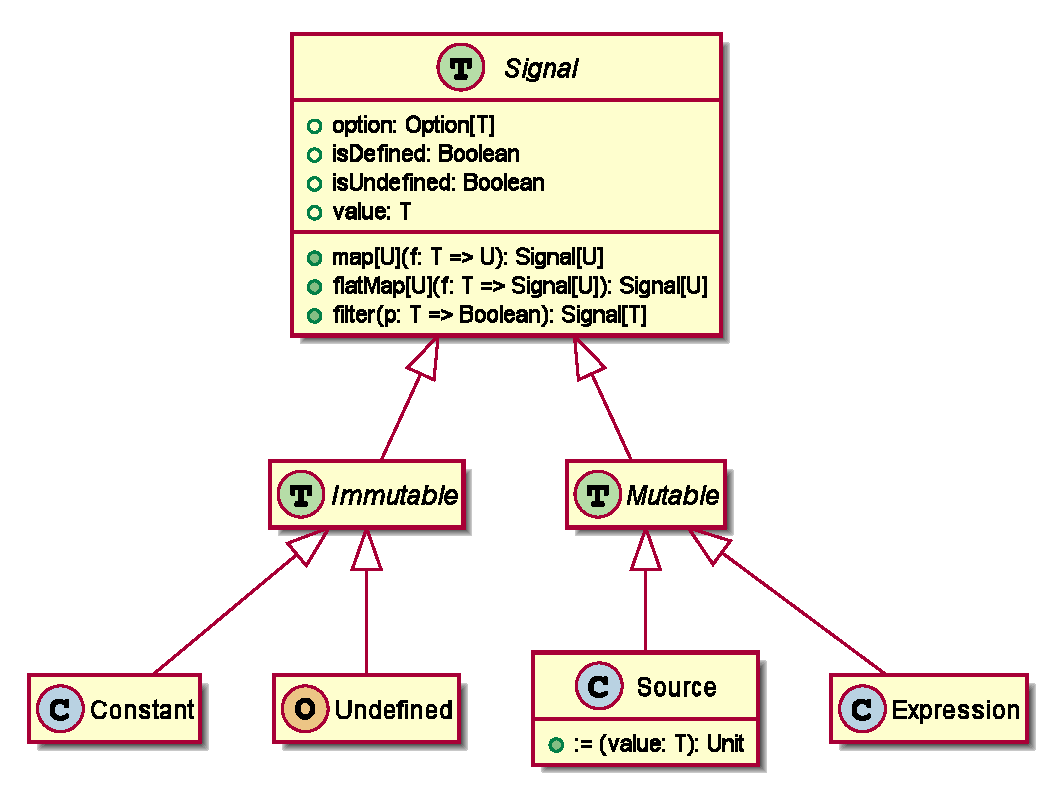
\includegraphics[width=12cm]{img/signals_simple}
	\caption{Hiérarchie simplifiée des signaux}
	\label{fig:sig-simple-hierarchy}	
\end{figure}

Le trait racine \texttt{Signal} est l'interface générique destinée à être manipulée par le développeur, quelque soit le type concret de signal manipulé. Il expose les méthodes nécessaires à l'accès à l'état courant du signal ainsi qu'à la construction de signaux dérivés par transformation. C'est une interface immutable qui ne permet de modifier l'état courant du signal.

La séparation des signaux en deux sous-arbres --- \texttt{Mutable} et \texttt{Immutable} --- capture les différences sémantiques liées à la présence ou l'absence d'une garantie d'immutabilité de l'état d'un signal.

L'intérêt d'un signal dont la valeur ne varie pas peut sembler limité à priori mais se présente lorsqu'une valeur non-signal doit être encapsulée dans un signal afin de satisfaire le système de types. Un tel signal n'a pas de raison de changer d'état au fil du temps, il est alors effectivement immutable. La présence de cette contrainte de façon explicite au niveau de la hiérarchie permet la mise en place d'un certain nombre d'optimisations.

Une instance de la classe \texttt{Constant[T]} est simplement une valeur de type \texttt{T} avec une interface de signal. Un tel signal est toujours dans l'état \emph{défini}.

L'objet singleton \texttt{Undefined} représente quant à lui le signal dont l'état est toujours \emph{indéfini}. Il est généralement référencé à partir de l'objet compagnon du trait \texttt{Signal}: sous la forme \texttt{Signal.undefined}. Puisqu'il n'est jamais défini, il est défini comme une instance de \texttt{Signal[Nothing]}, il est donc par covariance substituable à n'importe quel type de signal \texttt{Signal[T]} \footnote{\texttt{Nothing} est le \emph{bottom type} du système de types en Scala, il est sous-type de tous les types ($\forall \texttt{T}, \texttt{Nothing <: T}$) mais il n'en existe aucune instance.}.

Un signal immutable ne peut être ni \emph{enfant} ni \emph{parent} d'autres signaux. Comme ils ne changent jamais, il n'y a pas de sens de maintenir de graphe de dépendances entre eux. Il n'y aura en effet jamais de propagation de changement d'état à effectuer.

Les opérations de transformation --- \texttt{map}, \texttt{flatMap}, \texttt{filter}, etc. --- appliquées à des signaux constants sont évaluées immédiatement et produisent un nouveau signal constant. Par exemple:

\begin{lstlisting}
val a: Constant[Int] = Constant(2)
val b: Constant[Int] = a.map(_ * 2) // effectuée immédiatement
\end{lstlisting}

\begin{figure}
	\begin{lstlisting}
var i: Int = 0
def f(v: Int): Int = { i += 1; v * 2 }

// Immutable
val a: Constant[Int] = Constant(2)
val b: Constant[Int] = a.map(f)
assert(i == 1) // `f` est évaluée immédiatement

// Mutable
val c: Signal[Int] = Signal(2)
val d: Signal[Int] = c.map(f)
assert(i == 1) // `f` est évaluée de façon paresseuse
assert(d.value == 4) // accès à l'état de `d`, évaluation
assert(i == 2)

// Une sémantique peut en cacher une autre...
val e: Signal[Int] = Constant(2) // typé `Signal`
val f: Signal[Int] = c.map(f)
assert(i == 3)
	\end{lstlisting}
	\caption{Exemple d'évaluation immédiate des transformations}
	\label{fig:constant-eager-transform}
\end{figure}

La figure \ref{fig:constant-eager-transform} illustre ce comportement de façon plus explicite par l'introduction d'effets de bord dans la fonction de transformation utilisée. Cet exemple souligne également l'importance de la pureté des fonctions utilisées en pratique.

Les deux types de signaux mutables, sources (§ \ref{sec:sig-source}) et expressions (§ \ref{sec:sig-expr}), sont décrits plus en détails dans les sections les concernant.

\subsection{Construction}
Un signal est généralement dérivé par transformation de signaux existants. Cependant, dans le cas où un nouveau signal racine doit être construit, deux approches sont disponibles.

La première méthode est l'utilisation des constructeurs offerts par l'objet \texttt{Signal}:

\begin{itemize}
	\item \code{def Signal.apply[T](expr: => T): Signal[T]}
	\item \code{def Signal.define[T](expr: => Option[T]): Signal[T]}
\end{itemize}

L'expression fournie à \texttt{apply} sera évaluée pour déterminer la valeur du signal produit et les dépendances vers d'autres signaux seront automatiquement identifiées. Si l'expression fait référence à l'état d'au moins un signal parent non-constant, un signal de type \texttt{Expression} (§ \ref{sec:sig-expr}) est retourné. Dans le cas où aucun signal parent n'a été accédé, un signal de type \texttt{Constant} est retourné.

La variante \texttt{define} est similaire mais considère une valeur \texttt{None} comme un signal indéfini tandis qu'une valeur \texttt{Some(v)} est considérée comme un signal défini et de valeur \texttt{v}. 

La secondes approche consiste en l'utilisation explicite d'un signal de type \texttt{Source} (§ \ref{sec:sig-source}). 

\subsection{Signal source} \label{sec:sig-source}

Une \texttt{Source[T]} est l'équivalent réactif d'une variable en programmation non-réactive. C'est un conteneur mutable pour une valeur de type \texttt{T}, pouvant être indéfinie. Deux constructeurs sont disponibles selon l'état initial désiré pour la source:

\begin{itemize}
	\item \code{def Source.apply[T](value: T): Source[T]}
	\item \code{def Source.undefined[T]: Source[T]}
\end{itemize}

Une instance de \texttt{Source[T]} offre une méthode de mutation explicite
\begin{center}
	\code{def := (value: T): Unit}
\end{center}
permettant de mettre à jour la valeur contenue dans la source de façon impérative. Cette opération est un changement d'état de la source et provoquera l'invalidation récursive des tous les signaux en dépendant.

Une source est destinée à être utilisées lors de la construction de système hybrides, combinant code impératif basé sur les effets de bords et code fonctionnel. La source est alors un point d'entrée dans le graphe de dépendances des signaux pour la partie de code impérative.

\textit{À ajouter: une opération utilisant une fonction de mutation à partir de l'état courant:}
\begin{lstlisting}
	def ~= (f: T => T): Unit = { this := f(value) }
\end{lstlisting}

\subsection{Signal expression} \label{sec:sig-expr}

Un signal expression est un signal dont la définition est une expression arbitraire. Un tel signal détermine automatiquement ses signaux parents en observant les signaux accédés lors de l'évaluation de l'expression et construit ainsi automatiquement son arbre de dépendances. Si l'un de ces signaux venait à changer, la valeur du signal expression serait recalculée.

Il est construit en passant l'expression de définition au constructeur \texttt{Signal} tel qu'illustré par la figure \ref{fig:signal-expr-init}. La variante \texttt{Signal.define} est similaire à la méthode \texttt{apply}, mais reçoit une expression de type \texttt{Option[T]}. Une évaluation de cette expression produisant la valeur \texttt{None} ou une instance \texttt{Some(v)} conduit respectivement à un état indéfini ou défini du signal.

\begin{figure}[!h]
	\begin{lstlisting}
val a: Signal[Int] = ...
val b: Signal[Int] = ...
val c: Signal[Int] = Signal {
	a.value + b.value
}
	\end{lstlisting}
	\caption{Déclaration d'un signal expression}
	\label{fig:signal-expr-init}
\end{figure}

Les parents d'un signal expression sont dynamiques. À chaque évaluation, la liste des parents est vidée puis reconstruite selon l'évaluation actuelle. De cette façon, les dépendances sont toujours le plus précises possible et les invalidation inutiles sont évitées. Ceci est particulièrement important dans le cas de signaux contenant des branches et donc un ensemble de dépendances dynamiques selon l'état d'autres signaux.

Dans l'exemple de la figure \ref{fig:signal-expr-branches}, le signal construit ne dépend de \texttt{b} que si la valeur du signal \texttt{a} est \texttt{false}. Dans le cas contraire, il est dépendant de \texttt{c}. Dans tous les cas, une dépendance est créée vers le signal \texttt{a}.

\begin{figure}[!h]
	\begin{lstlisting}
Signal {
	if (a.value) b.value else c.value
}
	\end{lstlisting}
	\caption{Définition d'un signal expression avec branches}
	\label{fig:signal-expr-branches}
\end{figure}

Selon la situation, l'usage d'une expression pour définir un signal peut se révéler plus simple que la combinaison de nombreuses opérations de transformations élémentaires pour composer le comportement attendu.

Dans les cas les plus complexes, principalement lors de l'utilisation de structures de contrôles tel que des branches conditionnelles, des opérations de \emph{pattern matching} ou des boucles, une expression permet une définition concise et atomique du signal tandis que pour obtenir un résultat équivalent à l'aide des opérateurs de transformation, une longue chaîne de transformations successives, considérablement plus difficile à comprendre, serait nécessaire.

À l'inverse, dans les cas plus simples, une opération de transformation permet de réutiliser un \emph{pattern} de transformation établi, étant alors à la fois plus concis et mentalement plus simple puisqu'il utilise une sémantique clairement établie et commune.

\subsubsection{Contraintes des expressions}

Les signaux doivent être considérés comme des constructions semi-pure d'un point de vue fonctionnel (§~\ref{sec:sig-pureness}). Il est ainsi important que l'expression utilisée comme définition respecte ce principe en ne provoquant aucun effet de bord et en ne dépendant d'aucune valeur mutable qui ne serait pas un signal. En effet, si une valeur mutable non-signal est référencée par une expression, l'état résultant du signal est alors dépendant de l'instant d'évaluation pour lequel aucune garantie n'est fournie.

Il est aussi important que l'évaluation d'une expression s'effectue de façon synchrone. En effet la liste de dépendances du signal est construite lors de l'évaluation de l'expression. Si un signal parent est accédé de façon asynchrone ou \emph{lazy}, la dépendance ne sera pas identifiée et le signal ne sera pas correctement invalidé en cas de changement d'état de ce signal parent.

Les deux principaux suspects à considérer sont \texttt{Future} et \texttt{Stream}. Le premier pour le délai qu'il introduit dans l'évaluation de sa valeur, le second pour sa sémantique \emph{lazy}.

Il est intéressant de noter que la seule observation du paramètre de type du signal permet d'identifier un potentiel problème. En effet un signal de type \texttt{Signal[Int]} dont la définition impliquerait l'utilisation d'une instance de \texttt{Stream} n'est pas un souci; une fois la valeur finale de type \texttt{Int} produite, l'ensemble des éléments pertinents du flux auront été consommés de façon synchrone. Le principe s'applique de façon similaire à l'opération \texttt{Option.orElse} pour laquelle le paramètre est passé \emph{by name}.

À l'inverse, un signal \texttt{Signal[Stream[Int]]} expose l'instance de \texttt{Stream} utilisée. Dans une telle situation, si le calcul d'un élément du flux requiert l'accès à un autre signal, aucune relation de dépendance ne sera établie. Des types de signaux tels que \texttt{Signal[Stream[A => B]]}, \texttt{Signal[Future[A]]} voir même \texttt{Signal[A => B]} indiquent un risque important ne pas respecter la contrainte de synchronisme.

\subsection{Opérateurs de transformations}
Dans les exemples ci-dessous, les opérations sont supposées appliquées à une instance de type \texttt{Signal[T]}, \texttt{T} faisant ainsi référence au type d'élément contenu dans le signal original. Seules les opérateurs les plus courants et ceux utilisées par le compilateur Scala lors de la compilation d'une compréhension \texttt{for} sont traités ici. La Scaladoc du projet contient une liste exhaustive des opérations disponibles.

\subsubsection{Opérateur de transformation simple (\texttt{map})}

\begin{itemize}
	\item \code{def map[U](f: T=>U): Signal[U]}
\end{itemize}

La fonction \texttt{map} effectue une opération de transformation simple sur la valeur d'un signal en appliquant la fonction \texttt{f} à la valeur courante du signal et retournant un nouveau signal contenant en tout temps le résultat de cette transformation. En d'autre termes, lorsque l'état du signal original change, la fonction \texttt{f} est réévaluée avec la nouvelle valeur du signal parent et le signal enfant est mis à jour.

Si le signal d'origine est indéfini, la fonction \texttt{f} n'est pas appliquée et le signal enfant prend également l'état indéfini.

\begin{figure}[h]
	\begin{lstlisting}
val a: Signal[Int] = Source(4)
val b: Signal[Double] = a.map(Math.sqrt(_)) // b.value -> 2.0
a := 9 // b.value -> 3.0

val c: Signal[_] = Signal.undefined // `c` est indéfini
val d: Signal[_] = c.map(value => ???)
d.option == None // la fonction passée à `map` n'est jamais évaluée
	\end{lstlisting}
	\caption{Exemple d'utilisation de \texttt{map}}
\end{figure}

\subsubsection{Opérateur de sélection (\texttt{flatMap})}

\begin{itemize}
	\item \code{def flatMap[U](f: T=>Signal[U]): Signal[U]}
\end{itemize}

Dans le cas des signaux, \texttt{flatMap} implémente une opération de sélection: étant donné un signal \texttt{a} de type \texttt{Signal[T]} et une transformation sous la forme d'une fonction \texttt{f: T => Signal[U]}, la fonction \texttt{f} est appliquée à la valeur actuelle du signal \texttt{a} afin d'obtenir un second signal \texttt{b} de type \texttt{Signal[U]} et retourne un troisième signal \texttt{c} également de type \texttt{Signal[U]} dont la valeur est en tout temps égale à celle du signal \texttt{b}. La fonction \texttt{f} est réévaluée à chaque changement d'état du signal \texttt{a} afin de définir un nouveau signal de référence \texttt{b}.

Si le signal \texttt{a} est indéfini, la fonction \texttt{f} n'est pas appliquée et le signal \texttt{c} est également considéré indéfini.

La fonction \texttt{flatMap}\footnote{\emph{bind} en Haskell, ou \texttt{>>=}} est la fonction universelle de transformation des monades. Elle est suffisamment générale pour permettre de définir toutes les autres fonctions de transformation comme des cas particuliers de \texttt{flatMap}. Par exemple, la transformation \texttt{a.map(f)} peut également s'écrire  sous la forme \texttt{a.flatMap(value => Constant(f(value))}.

\begin{figure}[h]
	\begin{lstlisting}
val choice: Signal[Int] = ...
def selectSignal(choice: Int): Signal[T] = ...
// L'état de `c` est identique à celui du signal retourné par `selectSignal` pour la valeur courante de `choice`
val c: Signal[T] = choice.flatMap(selectSignal)
	\end{lstlisting}
	\caption{Exemple d'utilisation de \texttt{flatMap}}
\end{figure}

\subsubsection{Opérateur de filtrage (\texttt{filter})}

\begin{itemize}
	\item \code{def filter(p: T=>Boolean): Signal[T]}
\end{itemize}

La fonction \texttt{filter} effectue une opération de filtrage d'un signal en appliquant un prédicat \texttt{p} à la valeur courante du signal et retournant un nouveau signal de même valeur si le prédicat est vérifié, ou un signal indéfini si le prédicat n'est pas vérifié.

\begin{figure}[h]
	\begin{lstlisting}
	val a: Signal[Int] = Source(4)
	val b: Signal[Int] = a.filter(_ % 2 == 0) // b.option -> Some(4)
	a := 5 // b.option -> None, b.value -> UndefinedSignalException
	\end{lstlisting}
	\caption{Exemple d'utilisation de \texttt{filter}}
\end{figure}

\subsubsection{Opérateur de combinaison (\texttt{fold} / \texttt{reduce})} \label{sec:sig-op-fold}

\begin{itemize}
	\item \code{def fold[U](a: U)(f: (U, T)=>U): Signal[U]}
	\item \code{def reduce[U >: T](f: (U, T)=>U): Signal[U]}
\end{itemize}

L'opérateur \texttt{fold} permet l'introduction d'un effet de \emph{mémoire} aux signaux. Il prend en paramètre un \emph{accumulateur initial} \texttt{a} de type \texttt{U} et une fonction de combinaison \texttt{f: (U, T) => U} permettant d'associer la valeur courante du signal à cet état pour produire un \emph{accumulateur courant}, également de type \texttt{U}, qui sera alors la valeur du signal produit par l'opérateur.

Lors d'un changement d'état du signal initial, l'\emph{accumulateur antérieur} est combiné à la nouvelle valeur du signal pour former le nouvel \emph{accumulateur courant}. Si le signal est indéfini la fonction \texttt{f} n'est pas évaluée et l'\emph{accumulateur antérieur} devient l'\emph{accumulateur courant} sans modification. Dans le cas où le signal est initialement indéfini, l'\emph{accumulateur initial} devient l'\emph{accumulateur courant} tel quel.

Le signal retourné par \texttt{fold} est toujours défini.

L'opérateur \texttt{fold} possède la particularité d'être affecté par le mode d'évaluation du signal qu'il produit. En mode paresseux, l'opérateur de combinaison ne serait appliqué que lors de l'accès au signal enfant. Il serait alors possible de \emph{manquer} des changements d'état du signal parent. C'est pourquoi les signaux produits par l'opérateur \texttt{fold} ont toujours un mode d'évaluation strict afin d'obtenir un comportement déterministe et indépendant de la façon dont le signal enfant est utilisé.

À l'inverse de la fonction \texttt{fold} présente sur les collections de la bibliothèque standard Scala qui retourne une unique valeur pour une collection. La fonction \texttt{fold} des signaux retourne également un \texttt{Signal}. Le nom \emph{fold} ne fait ainsi pas référence au passage d'une collection à un élément unique, mais à la combinaison successive des différents \emph{états} du signal parent.

\begin{figure}[h]
	\begin{lstlisting}
val a: Signal[Int] = ...
val s: Signal[Int] = a.fold(0)(_ + _)
// Le signal `s` représente la somme de toutes les valeurs du signal `a`.

val b: Signal[Int] = ...
val m: Signal[Int] = b.fold(0)(_ max _)
// Le signal `m` représente la valeur maximale obtenue par le signal `b`.
	\end{lstlisting}
	\caption{Exemple d'utilisation de \texttt{fold}}
\end{figure}

L'opérateur \texttt{reduce} est une variation de l'opérateur \texttt{fold} dont l'\emph{accumulateur initial} est déterminé implicitement par l'état courant du signal parent. À l'inverse de la transformation \texttt{fold}, si l'état courant du signal parent est indéfini, alors le signal enfant est également indéfini. Dès lors que l'état du signal parent sera défini pour la première fois, l'état du signal enfant ne pourra plus être indéfini.

\begin{figure}[h]
	\begin{lstlisting}
val a: Signal[Int] = ...
val b: Signal[Int] = a.reduce((acc, x) => x)
// La valeur du signal `b` reflète la valeur du signal `a` lorsque celui-ci est défini. Lorsqu'il est indéfini, le signal `b` contient la dernière valeur définie du signal `b`. Si `a` n'a jamais été défini, `b` est indéfini.

val c: Signal[Int] = ...
val d: Signal[Int] = c.reduce(_ max _)
// Similaire à l'exemple correspondant pour `fold`, mais ne suppose pas une valeur intiale de 0. Si `c` représente des nombres négatifs, la version avec `fold` ne serait pas correcte (il faudrait utiliser Int.MinValue).
	\end{lstlisting}
	\caption{Exemple d'utilisation de \texttt{reduce}}
\end{figure}

\textit{À DÉTERMINER: Initialement, une variante \texttt{foldLazy} était envisagée qui produirait un signal avec le mode d'évaluation lazy. Dans quelles situations serait-ce adapté? J'avais initialement en tête des opérateurs tels que \texttt{max} qui ne conserve pas de trace de la séquence observée mais seulement un unique élément. Mais même de tels opérateurs n'ont pas de sens en évaluation paresseuse. L'essence de l'opération \texttt{fold} est de combiner des états successifs, comment cette opération peut-elle avoir un sens si certains états sont manqués de façon non-prévisible?}

\subsubsection{Opérateurs d'encapsulation (\texttt{wrap / unwrap})}

\begin{itemize}
	\item \code{def wrap: Signal[Option[T]]}
	\item \code{def unwrap[U](implicit ev: T <:< Option[U]): Signal[U]}
\end{itemize}

L'opérateur \texttt{wrap} transforme un signal d'origine de type \texttt{T} en un signal de type \texttt{Option[T]}. Lorsque le signal initial est défini, ce nouveau signal sera défini à \texttt{Some(value)}, avec \texttt{value} la valeur actuelle du signal original. Dans le cas où il serait indéfini, le signal de retour est défini à \texttt{None}.

Cette opération garantit ainsi un signal toujours défini à une instance d'\texttt{Option} et permet de contourner la sémantique des opérateurs de transformations vis-à-vis des signaux indéfinis. Ceci permet de traiter avec des opérateurs tel que \texttt{map}, \texttt{fold}, etc., les valeurs définies mais également indéfinies d'un signal.

\begin{figure}[h]
	\begin{lstlisting}
// Construction d'un signal avec une valeur par défaut qui sera utilisée si le signal original est indéfini
def withDefault[U >: T](s: Signal[T]])(default: U): Signal[U] = {
	val a: Signal[Option[T]] = s.wrap
	a.map((opt: Option[T]) => opt.getOrElse(default))
}
	\end{lstlisting}
	\caption{Exemple d'utilisation de \texttt{wrap}}
\end{figure}

L'opération \texttt{unwrap} effectue la transformation inverse. Si le signal initial possède une valeur \texttt{Some(v)}, la valeur du signal retourné est simplement égale à \texttt{v}. Dans le cas où le signal original vaut \texttt{None}, le signal résultant est indéfini. Cette opération ne peut être appliquée que sur une instance de signal de type \texttt{Signal[Option[U]]} pour un \texttt{U} quelconque.

Le paramètre implicite n'est rien d'autre qu'une implémentation de cette contrainte \footnote{La même technique est utilisée par les collections de Scala pour l'implémentation de la méthode \texttt{flatten}.}. Si celle-ci est respectée, le compilateur Scala sera en mesure de fournir une valeur pour ce paramètre implicite. En revanche, si le type du signal ne correspond pas, une erreur de compilation liée à l'absence du paramètre implicite sera générée. Le développeur n'a donc pas à se soucier de ce paramètre implicite et peut se contenter d'utiliser cette méthode tel que si elle ne prenait aucun paramètre.

\begin{figure}[h]
	\begin{lstlisting}
// Définition de l'opérateur `reduce` à partir de `fold` et `unwrap`
def reduce[U >: T](s: Signal[T])(op: (U, T) => U): Signal[U] = {
	val a: Signal[Option[U]]] =
		s.fold[Option[U]](None) { (prev: Option[U], cur: T) =>
			prev.map(op(_, cur))
		}
	a.unwrap
}
	\end{lstlisting}
	\caption{Exemple d'utilisation de \texttt{unwrap}}
\end{figure}

\subsection{Observateurs} \label{sec:sig-obs}

Les observateurs permettent d'ajouter des effets de bords aux changements d'états d'un signal. De la même façon que les sources sont les points d'entrée dans un graphe de signaux, les observateurs sont les points de sorties.

{\itshape

Les observateurs ne sont pas encore implémentés au niveau de la bibliothèque. Quelques propriétés prévues:
\begin{itemize}
	\item Un observateur possède un ensemble de signaux qu'il observe
	\item Il est invoqué lorsque l'état d'un de ces signaux change
	\item Détection dynamique des signaux observés de façon similaire aux signaux expression; l'ensemble des signaux observés peut varier au cours du temps.
	\item Un observateur peut être désactivé pour le déconnecter du graphe de signaux
	\item Il peut être réactivé par la suite
	\item Appelé de façon asynchrone à la fin d'un contexte de mutation atomique, avec la sémantique exactly-once.
\end{itemize}



Les blocs \texttt{atomically} peuvent être nestés, auquel cas ils n'ont aucun effet hormis pour le bloc le plus extérieur. La mutation d'une source est toujours associée à un contexte de mutation, il n'est donc pas nécessaire d'en définir un explicitement lors de la modification d'une seule valeur.

}

\subsection{Contexte de mutations atomiques}
\textit{Ce concept est relativement récent dans mon développement, il est destiné à supporter l'implémentation des observateurs et à fournir une structure de base pour les mécanismes de thread-safety.}

Un contexte de mutations est un bloc à l'intérieur duquel les changements apportés à un graphe de signaux sont appliqués de façon atomiques. Il prend la forme d'une construction de la forme:
\begin{lstlisting}
Signal.atomically {
	// mutations...
}
\end{lstlisting}

Aucun observateur n'est invoqué jusqu'à la sortie du bloc \texttt{atomically}. Il est ainsi possible d'effectuer une série de mutations dans un graphe de signaux et de ne notifier les observateurs qu'une seule fois à la fin.

Ces blocs peuvent être imbriqués, dans ce cas, les blocs intérieurs n'ont pas d'effet et seul le bloc extérieur est considéré.

Le bloc \texttt{atomically} joue aussi un rôle dans l'évaluation des signaux stricts. Ceux-ci ne sont en effet recalculés qu'une seule fois à la fin du bloc, mais avant l'invocation des observateurs. Une exception existe cependant: si l'état d'un signal strict est accédé explicitement à n'importe quel moment à l'intérieur du bloc, cet état sera calculé immédiatement.

\textit{À ajouter: exemples}


\subsection{Parallélisme}
\textit{La question du parallélisme reste ouverte pour l'instant. Deux cas à considérer:}
\begin{enumerate}
	\item \emph{Utilisation multi-thread d'un unique graphe de signaux}: implique une gestion correcte de la concurrence afin de garantir un état cohérent du graphe en tout temps ainsi que d'éviter de potentiels inter-blocages lors du calcul parallèle de plusieurs branches du graphe. Il est aussi important de définir clairement la sémantique des observateurs dans le contexte multi-thread. Quel est le thread exécutant l'observateur? En cas de modification concurrente, combien d'appels à l'observateur? Une invocation unique une fois le graphe stabilisé entre tous les threads? Une invocation (exactement ou au plus ?) par thread?
	\item \emph{Signaux comme mécanisme de parallélisation}: dans cette situation le graphe de signaux est considéré comme une fonction utilisée pour paralléliser automatiquement un traitement. Une source est définie pour chaque paramètre et des transformations de signaux sont utilisées pour réaliser les étapes intermédiaires de l'algorithme. Le résultat prend la forme d'un signal unique en bas de l'arbre de dépendances. Dans une telle configuration, le calcul des signaux indépendants peut être parallélisé de façon automatique (utilisation d'un thread pool géré par le framework?). L'ensemble peut alors être exposé sous la forme d'une fonction \texttt{(A, B, C, ...) => Future[Z]}. Utilisant un observateur sur le noeud final pour résoudre les futures retournés.
	
	Il est de plus intéressant de noter que si le premier cas d'utilisation parallèle est implémenté avec une sémantique \emph{exactly-once} cohérente au niveau des observateurs, le graphe utilisé par la fonction peut alors être utilisé par plusieurs thread simultanément et former un \emph{pipeline} de calcul dans lequel il est possible de débuter un nouveau calcul dès lors que l'ensemble des noeuds directement dépendant des signaux sources ont été évalués. Et ainsi de suite pour les signaux de niveau suivants. Allons-nous aller jusque là?
\end{enumerate}

\textit{Il n'est pas clair quels développements seront entrepris dans le domaine du parallélisme, l'implémentation actuelle est basée sur une approche single-thread adaptée à un usage dans le navigateur. L'intérêt pour ce projet étant plus sur au niveau de la propagation automatique des mises à jour que sur le parallélisme du calcul.}




\section{Solutions existantes}

\subsection{ReactiveX}
Dans les implémentations les plus populaires de framework réactifs-fonctionnels, dont notamment la bibliothèque \emph{ReactiveX} disponible pour de nombreux langages, on retrouve généralement un concept similaire sous le nom de \texttt{Rx}.

Bien que tous deux soient une abstraction du temps, les \texttt{Rx} représentent fondamentalement une séquence tandis qu'un \texttt{Signal} est une valeur unique à un instant donné. Afin de clarifier cette distinction, ces deux interfaces peuvent être comparées à leur équivalent non-réactif le plus proche dans la bibliothèque standard de Scala:

\begin{table}[H]
	\begin{tabular}{@{}p{2.5cm}p{2.5cm}p{\dimexpr\textwidth-6cm\relax}@{}}
		\toprule
		Type de base & Type réactif & Différence \\ \midrule
		\texttt{Stream[T]} & \texttt{Rx[T]} & Tous les éléments d'un \texttt{Stream} sont calculables à l'instant présent, les éléments d'une \texttt{Rx} ne sont peut être pas encore disponibles \\
		&  & \\
		\texttt{Future[T]} & \texttt{Signal[T]} & Un \texttt{Future} n'est résolu qu'une seule fois, un \texttt{Signal} peut changer de valeur de multiples fois au cours du temps \\ \bottomrule
	\end{tabular}
\end{table}

Ainsi, certaines opérations monadique dont la sémantique peut être ambiguë dans le cas des valeurs réactives peuvent avoir des comportements considérablement différents entre ces deux concepts. C'est le cas notamment de la fonction \texttt{flatMap}
\footnote{\texttt{Signal[T].flatMap[U](fn: T => U): Signal[U]}, de façon similaire pour \texttt{Rx[T]}}:

\begin{itemize}
	\item Sur une valeur \texttt{Rx}, l'opération \texttt{flatMap} effectue une concaténation des valeurs des sous-séquences retournées, potentiellement entrelacées.
	\item Sur un \texttt{Signal}, l'opération \texttt{flatMap} se comporte comme un switch: le signal original est utilisé pour sélectionner un second signal, dont la valeur sera celle du signal produit par \texttt{flatMap}. Lorsque la valeur du signal initial change, la sélection est effectuée à nouveau et le signal résultant est utilisé comme nouvelle source de valeurs.
\end{itemize}

Bien que la bibliothèque \emph{ReactiveX} propose un opérateur spécifique avec la sémantique de switch, il est utile de préciser que l'opération \texttt{flatMap} est l'opération utilisée par le langage Scala lors de l'utilisation de multiples générateurs dans une compréhension \texttt{for}.

Ainsi le code
\begin{lstlisting}
val a: Signal[Int] = ...
val b: Array[Signal[Double]] = ...
val c: Signal[Double] = for (x <- a; y <- b(x)) yield y * 2
\end{lstlisting}

sera transformé par le compilateur en
\begin{lstlisting}
val c = a.flatMap(x => b(x)).map(y * 2)
\end{lstlisting}

et produira des résultats radicalement différents selon l'abstraction utilisée:

\begin{itemize}
	\item Dans le cas des \texttt{Rx}, le résultat est l'agglomération des tous les flux de valeurs de \texttt{b} sélectionnés au fil du temps, potentiellement de multiples fois. Le résultat n'est très probablement pas celui escompté.
	
	\item Dans le cas de \texttt{Signal}, le résultat est un signal \texttt{c} dont la valeur est le double de celle d'un signal contenu dans le tableau \texttt{b} et désigné par la valeur du signal \texttt{a}, le tout sur la base des valeurs de ces signaux au moment présent. Dans le future, lorsque la valeur de \texttt{a} ou de \texttt{b(x)} changera, la valeur de \texttt{c} sera également mise à jour.
\end{itemize}

La sémantique des signaux, basée sur les valeurs plutôt que la séquences de ces valeurs, a pour but d'être la plus adaptée possible à l'usage qui en est fait dans ce travail, c'est à dire la conception d'interfaces graphique.

Une conséquence supplémentaire de cette différence entre signaux et \texttt{Rx} est la possibilité de définir aisément le concept de \emph{signal expression} dans le cas des signaux. Dans le cas des \texttt{Rx}, le comportement attendu d'une telle construction n'est pas évident dans une situation où les flux sont potentiellement finis.

\subsection{Scala.rx}
Scala.rx est l'implémentation la plus proche des signaux utilisés dans ce projet. La simplicité d'utilisation est particulièrement appréciable avec la méthode de définition de \texttt{Rx}s sur la base d'expressions arbitraires.

Les différences sont principalement liées aux limitations volontairement imposées dans Scala.rx.

\subsubsection{Pas de variable réactive non-définie / vide}
La raison invoquée est la difficulté d'intégrer l'absence de valeur de façon intuitive dans la syntaxe déclarative. Plus spécifiquement, l'auteur mentionne plusieurs solutions potentiels:
\begin{enumerate}
	\item Bloquer le thread courant jusqu'à ce qu'une valeur soit disponible. Cette solution n'est cependant pas envisageable pour une implémentation visant l'environnement Javascript.
	\item Lancer une exception lors de l'accès à une variable vide, mais recommencer l'opération une fois que sa valeur sera définie. Cette option présente le désavantage que le calcul d'une variable réactive puisse potentiellement être démarré puis interrompu de multiples fois si de nombreuses dépendances sont indéfinies.
	\item Obliger le style monadique et retirer la méthode implicite de définition. Cette option n'est pas considérée pour des raisons d'expérience utilisateur évidentes.
	\item Utiliser un plugin du compilateur pour transformer automatiquement le code en style monadique. Cette approche présente cependant de nombreux défis techniques et requiert une étape supplémentaire de configuration indésirable.
\end{enumerate}

En pratique l'absence de variable réactive vide est une gêne considérable dans le domaine du web où toutes les opérations sont asynchrones et non-bloquante. Le concept de promesse est omni-présent et il est ainsi difficile d'associer les interfaces natives du navigateur avec le réseau de variables réactives.

Une première approche est d'utiliser directement le type \texttt{Option} de Scala pour exprimer l'absence d'information le temps de l'opération. Mais cette idée impose une verbosité beaucoup plus importante du code puisqu'il est maintenant nécessaire de manipuler explicitement des \texttt{Rx[Option[T]]} au lieu de simples \texttt{Rx[T]} et de laisser le soin de la gestion de l'asynchrone à la bibliothèque.

De plus, la seconde approche proposée (interrompre le calcul par une exception) ne semble pas déraisonnable et peut constituer une approche valide si correctement documentée. Il est important que les conséquences d'une variable indéfinie soient connues et considérées, mais leur absence volontaire semble au final plus gênante que bénéfique. Par ailleurs, le style monadique ne présente pas les inconvénients mentionnés et constitue une alternative valide si le style est plus adapté à un problème spécifique.

\subsubsection{Complexité de l'implémentation}
Malgré l'effort fourni pour proposer une interface simple et efficace, l'implémentation est en réalité relativement complexe et très largement basée sur l'utilisation de macros. Le code écrit par le développeur n'est pas le code finalement exécuté. Une raison probable de cette implémentation est basée sur la méthode choisie pour détecter automatiquement les dépendances entre variables réactives avec le style déclaratif.

Dans Scala.rx, les expressions qui définissent des variables réactives sont réécrite sous formes de fonctions exploitant largement le système de paramètres implicites pour transmettre le contexte d'accès à une variable réactive entre parent et enfant. Bien que cela soit une approche très proche des standards en Scala, elle requiert une couche syntaxique supplémentaire ou l'utilisation de macros afin de l'ajouter automatiquement. Le système résultant est excessivement complexe et les erreurs rencontrées lors de l'usage ne sont pas intuitives puisqu'elles ne correspondent pas au code écrit. 

De plus, l'approche n'est pas portable entre les versions de Scala puisqu'elle dépend de l'implémentation interne du compilateur. Dans le cas de Scala.rx, l'implémentation est compilée simultanément pour les version 2.10, 2.11 et 2.12 de Scala et requiert pour chaque version une implémentation différente des macros pour s'aligner avec les changements apportés au compilateur et à la syntaxe du langage.

Une approche alternative est possible: \texttt{DynamicVariable}. Cette classe de la bibliothèque standard de Scala est rarement utilisée puisque très spécifique et généralement moins explicite que l'usage de paramètres implicites qui sont plus en accord avec les principes de la programmation fonctionnelle. Elle rempli cependant un rôle semblable en offrant une sémantique de variable à portée dynamique plutôt que lexicale. Ce mécanisme permet de déplacer la transmission du contexte d'évaluation des paramètres implicites à un canal annexe dédié.

Le code est ainsi fortement simplifié puisque la transmission du contexte est clairement dissociée, évitant la nécessité de modifier le code utilisateur et donc l'usage de macros au prix d'une architecture pouvant être considérée moins pure d'un point de vue fonctionnel. L'absence de macros permet également une compatibilité plus aisée avec les futures versions du langage.

\subsubsection{Évaluation stricte}
\textit{Les \texttt{Rx}s de Scala.rx sont toujours évaluées de façon stricte. L'approche lazy des signaux de Xuen présente des avantages.}
\section{Implémentation}

\subsection{Hiérarchie complète}
\label{sec:sig-hierarchy}

La figure \ref{sec:sig-hierarchy} présente la hiérarchie formée par les différentes classes de signaux. Cette section aborde plus en détails les spécificités de chacune d'elles.

\begin{figure}[h]
	\centering
	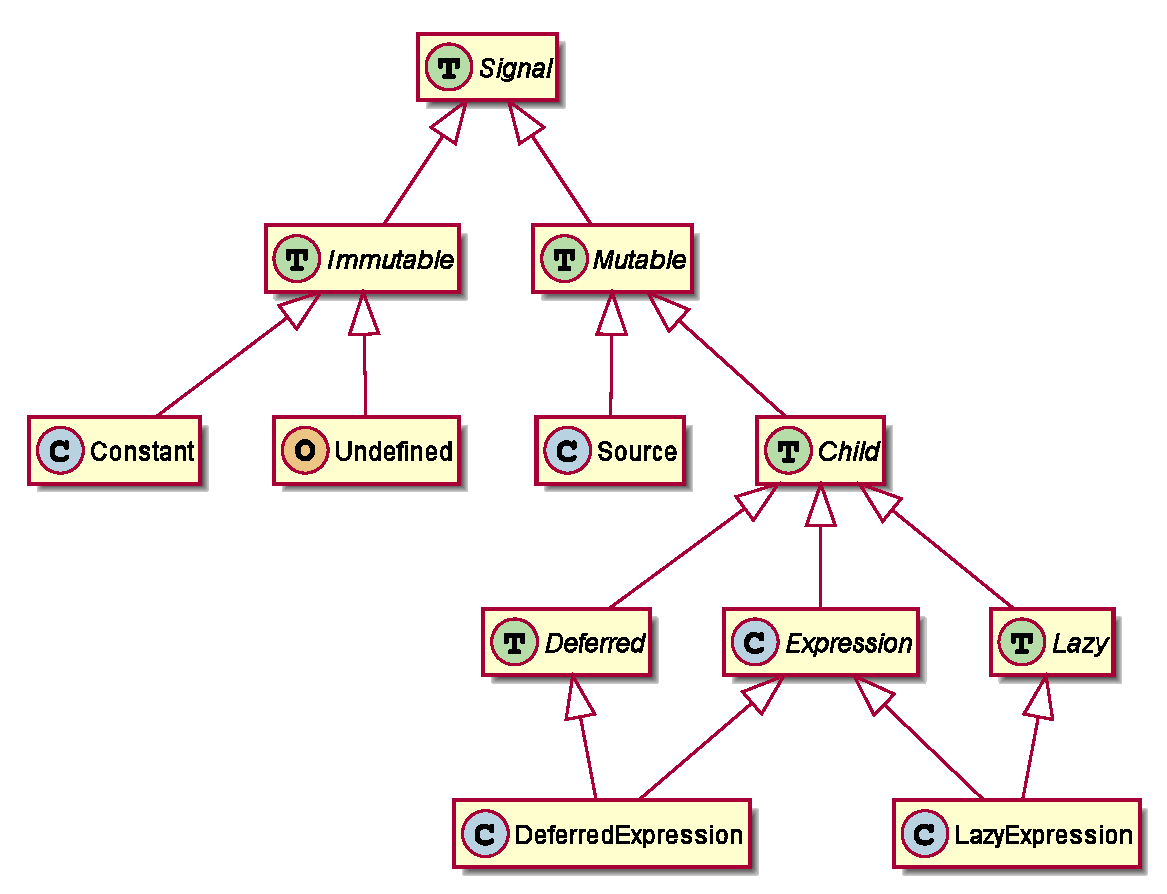
\includegraphics[width=10cm]{img/sig_hierarchy.eps}
	\caption{Hiérarchie des signaux}
	\label{fig:sig-hierarchy}
\end{figure}

\subsubsection{\texttt{Signal}}

Le trait racine de la hiérarchie expose les opérations communes à tous les signaux: accès à la valeur courante et opération de transformation. C'est une interface générique qui ne précise aucune sémantique particulière pour le signal. Elle est ainsi adaptée lorsque le type exact de signal manipulé n'est pas important, ce qui est généralement le cas.

\subsubsection{\texttt{Immutable}}

Cette première division distingue les signaux dont la valeur change au cours du temps de ceux pour lesquels la valeur reste constante.

\subsubsection{\texttt{Mutable}}

\subsubsection{\texttt{Lazy}}

\subsection{Implémentation des opérateurs monadiques}

\textit{CONTRAIREMENT À REACTIVEX, PAS DE CLASSES, MAIS UTILISATION DES EXPRESSIONS}

\subsection{Modèle push, pull ou hybride}

Deux modes de fonctionnement sont généralement décrit pour des systèmes fonctionnels-réactifs: \emph{push} et \emph{pull}.

L'approche \emph{push} se base sur les changements apportés aux signaux sources pour recalculer tous les signaux enfants qui en dépendent. Dans l'approche \emph{pull}, c'est l'accès aux signaux enfants qui provoque le calcul des valeurs intermédiaires jusqu'aux signaux sources. Dans les deux cas, des opérations potentiellement inutiles ou redondantes sont effectuées.

L'approche mixte \emph{push-pull} se base sur une approche principalement \emph{pull} où l'accès à l'état d'un signal déclenche son évaluation, auquel vient s'ajouter un mécanisme de \emph{mémoïsation} qui maintient l'état courant du signal après son calcul. L'invalidation de ces caches se fait ensuite selon une approche \emph{push}: un changement d'état des signaux sources est notifié à toutes les dépendances de façon récursive.

\textit{DEVELOPPEMENT DES AVANTAGES}

\subsection{Utilisation dans un environnement parallèle}

\textit{Pas de threads en JavaScript, donc un problème que côté serveur. Bien que le système fonctionne sur la JVM, il n'a pas été testé de façon étendue dans un contexte multi-thread; actuellement half-baked: les Signaux eux-même sont en principe thread-safe (aka invalidation / recalcul / etc) mais le système en entier n'est pas réellement étudié (dead-lock de signaux interdépendant?). Est-ce que utile au projet puisqu'on le use-case principal est celui du framework web côté client? Quid des observeurs et de la sémantique exactly-once pour une bloc de mutation atomic{} ?}


\chapter{Framework web}

\section{Motivations}
\textit{Construction d'un framework d'interface web sur la base des signaux introduits précédemment.}

\textit{Développement spécifiquement pour Scala.js. Il existe de nombreux bindings par exemple pour React ou Angular en Scala.js, mais l'utilisation d'un framework conçu pour JavaScript en Scala.js n'est pas toujours l'expérience la plus agréable. Volonté de disposer d'une API conçue pour le langage Scala.}

\textit{Transition signaux -> component (via template et data binding)}

\section{À propos des standards Web Components}

L'implémentation de la partie web de Xuen dépend extensivement des mécanismes introduits par les spécifications \emph{Shadow DOM} \cite{w3c-shadowdom}, \emph{Custom Elements} \cite{w3c-custom-elements} et les spécifications annexes telles que \emph{CSS Scoping} \cite{w3c-css-scopings}.

Ces standards définissent des mécanismes permettant la définition de nouveaux éléments personnalisés, encapsulés et réutilisables. Ils définissent également comment l'encapsulation du composant est implémentée au niveau des styles CSS et des événements DOM. Ces mécanismes sont réutilisés avec le minimum d'abstraction lorsque cela est possible pour Xuen.

Définir un élément Xuen (§ \ref{sec:web-specs-element}) correspond à la définition d'un nouvel élément \emph{Custom Elements}: la classe produite est passée à la méthode native \texttt{define()} du navigateur tel que le serait une classe construite directement en JavaScript.

Les templates se basent sur \emph{Shadow DOM} comme mécanisme d'encapsulation. Ils peuvent ainsi réutiliser le concept de \texttt{<slot>} introduit par ce standard comme primitive de composition. L'encapsulation standard des événements et des styles s'applique également.

Ces concepts sont répartis entre une multitude de spécifications, provenant de différentes organisations et peuvent être difficiles à aborder de prime abord. Néanmoins, une connaissance des ces mécanismes peut se révéler très utile à la compréhension de l'implémentation et du fonctionnement de Xuen.

En guise d'introduction, le guide \emph{Shadow DOM v1: Self-Contained Web Components} \cite{google-shadowdom} rédigé par Google dans la série \emph{Web Fundamentals} est un bon tour d'horizon des mécanismes liés à Shadow DOM.

\section{Spécifications} \label{sec:web-specs}

\textit{L'architecture du framework web est encore à un stade très primitif.}

\subsection{Composant}
\textit{Définition de nouveau composant. Un composant est défini par:}
\begin{itemize}
	\item \emph{Un sélecteur}: correspondant à la balise HTML qui sera définie pour ce composant. Ce nom doit comporter un tiret (selon la spécification \emph{Custom Elements}).
	\item \emph{Un template}: une structure HTML pouvant contenir des expressions de data-binding avec des données réactives sous la forme de signaux
	\item \emph{Une feuille de styles}: pouvant être utilisée pour définir l'apparence visuelle du composant
	\item \emph{Un behavior}: comportement de l'élément en réponses aux interactions. Implémentées en tant que classe Scala.js.
\end{itemize}

\subsection{Template}
\textit{Défini à partir de code HTML, il est parsé et compilé par le framework en un objet de type \texttt{Template} qui est alors utilisé pour chaque instance du composant.}

\textit{L'opération de compilation ne s'effectue qu'une seule fois à la première utilisation du composant puis réutilisé. La forme compilée et optimisée pour la création de nombreuses instances du template.}

\textit{Il y a donc un coût important lors de la première utilisation puis un coût minimal lors des utilisations futures, ce qui est cohérent avec l'utilisation des objets templates: définis une fois par composant, instantiés de nombreuses fois.}

\textit{Le template peut contenir des expressions de data-bindings qui seront utilisée pour y inclure dynamiquement des données provenant de signaux réactif.}

\subsection{Expressions}
\textit{La syntaxe des expressions est fortement inspirée des expressions de Angular 2, sémantiquement adaptée pour correspondre à une usage combiné aux signaux.}

\textit{Parser construit avec les "Parser Combinators" de Scala. Production d'un AST représentant l'expression puis optimisation de cet arbre.}

\textit{De façon similaire aux templates: coût initial important puis faible coût lors de l'utilisation.}

\textit{L'AST est passé à un interpréteur en même temps qu'une contexte d'évaluation spécifiant les variables globales à disposition est le composant dans lequel l'expression s'exécute.}

\textit{Peut être une section à part entière}

\subsection{Feuille de styles}
\textit{Simple morceau de code CSS qui sera injecté dans le sous-arbre Shadow DOM correspondant au composant.}

\subsection{Behavior}
\textit{Définition d'une classe Scala qui étend \texttt{XuenBehavior}, qui étend lui même l'interface DOM \texttt{HTMLElement}.}
\section{Solutions existantes}
\section{Implémentation}

\subsection{Vue d'ensemble}
\begin{figure}[h]
	\centering
	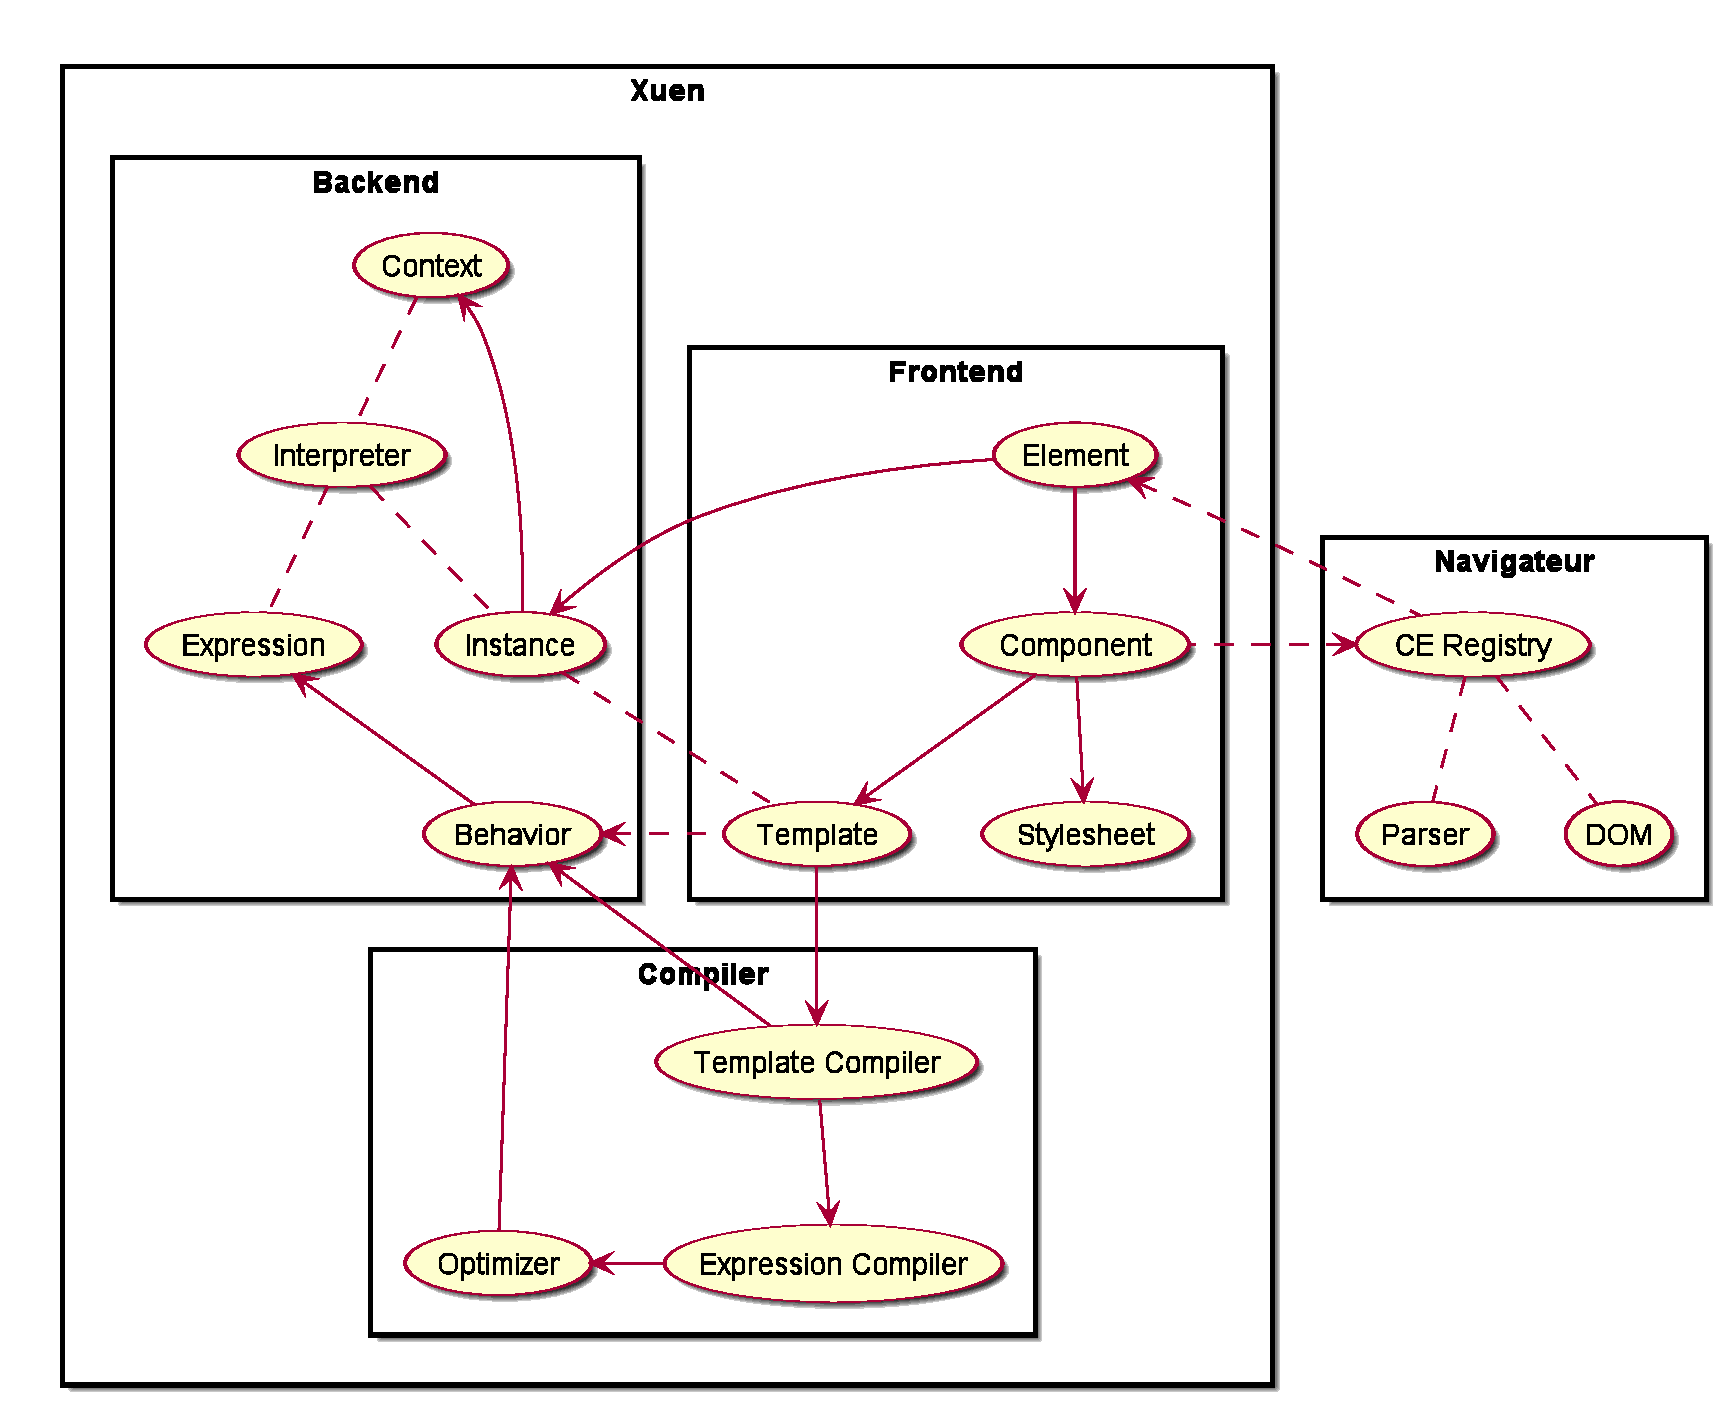
\includegraphics[width=\textwidth]{img/web_overview.eps}
	\caption{Vue d'ensemble de l'implémentation du framework Web}
	\label{fig:web-overview}
\end{figure}

L'implémentation du framework web de Xuen peut être décomposé en 3 grandes parties, tel qu'illustré par la figure \ref{fig:web-overview}.

\begin{enumerate}
	\item La partie \emph{front-end} est exposée directement au développeur. Elle est utilisée pour déclarer les composants personnalisés de l'application, leurs comportement et structure.
	\item La partie \emph{back-end} est utilisée par le framework lorsqu'un élément est instancié dans le document. Elle fournit les outils nécessaires à l'implémentation des comportements dynamiques du template de cet élément et l'interface avec le système de signaux par le biais des expressions.
	\item Finalement le système de compilation est utilisé lors de la définition d'un nouveau composant pour transformer le code source HTML du template en une instance de la classe \texttt{Template}, encapsulant à la fois une structure pré-traitée du template, des modèles pour construire les comportements dynamiques de ce template et des expressions sous forme d'arbres syntaxiques prêts à être interprétés.  
\end{enumerate}

L'objectif de la partie de compilation est de réduire l'impact du traitement du template au \emph{runtime}. En effet, l'instanciation d'un template se base sur les outils fournis par le navigateur, notamment le parser HTML et son implémentation du DOM afin parcourir et traiter la structure fournie sous forme de code HTML.

En compilant le template et les expressions dès la déclaration, il n'est plus nécessaire de le faire lors de l'instanciation, ce qui permet un investissement fixe au chargement de l'application et des performances accrues lors de son fonctionnement.

Cette structure est en grande partie reprise d'un projet personnel antérieur. La plupart des éléments ont été repensés et réimplémentés, principalement pour les adapter au nouveaux standards \emph{Web Components} version \emph{v1} (par opposition à la version antérieure \emph{v0}). Le parser d'expression a quant à lui été réécrit, passant d'une implémentation fortement inspirée du parser d'expression du framework Angular 2, mais en Scala, à une version développée avec la bibliothèque \emph{scala-parser-combinators} \cite{scala-parser-combinators}, plus propre et idiomatique. La grammaire du langage n'a cependant pas été significativement modifiée. L'optimisateur d'expressions est réutilisé pratiquement tel quel.

\subsection{Processus de compilation du template}

Le template est fourni à la bibliothèque sous forme de code source HTML. La première opération consiste donc à construire dynamiquement un élément \texttt{<template>} et à y insérer le code du développeur. Le parser HTML du navigateur sera alors invoqué pour construire une structure de nœuds DOM. Cette structure est ensuite parcourue de façon récursive en commençant à l'élément template créé précédemment.

\begin{itemize}
	\item Premièrement, la nature du noeud en cours est déterminée. S'il s'agit d'un nœud \texttt{Text} ou \texttt{Comment}, son contenu est scanné pour y identifier d'éventuelles interpolations.
	\item Si le nœud est un élément, ses attributs sont observés.
	\item Si l'élément est annoté d'une transformation \texttt{*if} ou \texttt{*for}, cette transformation est appliquée.
	\item Si l'élément possède des annotations de \emph{data-binding}, celles-ci sont traitées.
	\item Les valeurs des attributs restants qui ne sont ni des transformations ni des annotations de \emph{data-binding} sont scannées pour y identifier des interpolations.
	\item Une fois l'élément lui-même entièrement traité, l'ensemble de ses enfants est parcouru, réitérant le processus.
\end{itemize}

Pour chaque nœud DOM devant être associé à un comportement dynamique, un \texttt{Behavior} est créé. Celui-ci est identifié par un numéro incrémenté à chaque nouvelle instance. Il sera de modèle pour la construction du comportement dynamique en question. Tous les \texttt{Behavior}s créés pour un template son rassemblé dans une \texttt{Map} contenue dans l'objet \texttt{Template} resultant. L'élément auquel le comportement doit être attaché est quant à lui décoré d'un attribut \texttt{xuen:behavior="..."} indiquant l'identifiant du comportement associé à ce nœud.

Si l'élément ne peut pas posséder d'attribut, c'est à dire lorsqu'il s'agit d'un nœud \texttt{Text} ou \texttt{Comment}, un élément \emph{placeholder} \texttt{<xuen:placeholder>} est inséré à sa place dans l'arbre DOM du template et l'attribut est placé sur cet élément. Dans ce cas, lors de la construction du comportement au moment de l'instanciation du template, l'élément \emph{placeholder} sera en premier lieu remplacé par un nœud correspondant à l'original puis le comportement spécifique de ce nœud sera implémenté.

Un \texttt{Behavior} peut en réalité implémenter plus d'un comportement pour un même élément. Si deux annotations sont présentes sur un même élément, le \texttt{Behavior} construit à l'occasion du traitement de la première annotation est réutilisé pour la deuxième annotation. L'objet \texttt{Behavior} sera donc en charge de construire deux comportements dynamiques différents sur le même élément.

À l'inverse de la compilation, le processus d'instanciation est relativement simple. Le template est à présent sous forme normalisée, tous les comportements sont attachés à des éléments annotés par l'attribut \texttt{xuen:behavior}. Juste avant d'implémenter les comportements dynamiques, l'objet template est cloné pour construire une nouvelle structure indépendante de l'originale qui est conservée en tant que modèle. La bibliothèque utilise alors la \texttt{Map} associant les identifiants des différents comportements enregistrés avec les objets \texttt{Behavior} encapsulant la logique de construction pour instancier à proprement parler ces comportements.

Le sélecteur CSS \texttt{[xuen:behavior="..."]} est utilisé pour récupérer l'élément sur lequel le comportement doit être appliqué puis la méthode \texttt{build} de l'objet \texttt{Behavior} est invoquée avec la référence vers l'élément courant. Cette méthode va alors instancier à proprement l'ensemble des comportements liés à cet élément.

De façon générale \emph{instancier un comportement} implique construire une paire (signal, observateur) qui implémentera le comportement désiré. Cette paire est initialement construite déconnectée. Une fois l'élément hôte connecté, son template est \emph{activé} ce qui entraine la liaison  des observateurs avec le signal associé et donc la mise en place du comportement dynamique.

Lorsqu'un élément est déconnecté, son template est \emph{désactivé}. Cette opération déconnecte l'ensemble des signaux et observateurs utilisé dans l'implémentation de ce template, assurant ainsi qu'il n'existe plus de lien entre le reste du système et l'élément déconnecté. Sans cette étape, il existe un risque que les éléments ne puissent pas être désalloués par le \emph{garbage collector} puisqu'une référence subsiste entre le reste du graphe de signaux et eux.

\subsection{Ordre de construction des \emph{Custom Elements}}

La spécifique \emph{Custom Elements} \cite{w3c-custom-elements} défini très précisément la façon dont un élément personnalisé est initialisé par le navigateur. Cette procédure, appelée \emph{upgrade} \cite[\small 2.5 Upgrades]{w3c-custom-elements}, implique une combinaison de piles et de queues pour enregistrer les actions à effectuer par le navigateur au fil de l'analyse du document HTML.

De plus la notion de \emph{connexion} au document est introduite: un élément est \emph{connecté} si il fait partie de la hiérarchie du document, \emph{déconnecté} s'il s'agit d'un élément flottant hors de l'arbre DOM principal.

L'\emph{upgrade} d'un élément ne s'effectue en principe que si cet élément est \emph{connecté} au document. Sauf s'il s'agit d'un élément étant explicitement créé par l'utilisateur. Ainsi l'utilisation de la méthode \texttt{createElement} avec un élément personnalisé provoque l'\emph{upgrade} instantané de l'élément créé, mais laisse les éléments de son template dans l'état non-\emph{upgradé}, car ceux-ci n'ont pas été instancié explicitement et que leur parent, en l'occurrence l'élément créé par \texttt{createElement}, n'est pas encore inséré dans le document; ils ne sont donc pas considérés \emph{connectés}.

Le constructeur de l'élément racine est donc invoqué alors que le constructeur de ses enfants n'a pas encore été invoqué. Hors, il est déjà possible d'utiliser \texttt{querySelector} pour accéder à ces éléments non-initialisés.

Le problème s'amplifie lorsque l'élément parent devient \emph{connecté}. Le mécanisme de queues décrit dans le standard implique que l'appel du \emph{callback} de l'élément parent est planifié avant la considération des éléments enfants. Par conséquent, la méthode \texttt{connecteCallback} est invoquée sur l'élément parent, une fois encore, avant que ses enfants n'aient eu l'occasion de s'initialiser.

Dans Xuen, le \emph{callback} de connexion est utilisé pour activer le template de l'élément parent, construisant alors l'ensemble des liens de \emph{data-binding} entre parent et enfants. Si un élément enfant n'est pas encore instancié à ce moment là, les points de connexion sous forme de signaux permettant le \emph{data-binding} ne sont pas encore disponibles et le système est alors laissé dans un état totalement inutilisable.

Afin de contourner ce problème, l'initialisation d'un élément personnalisé place temporairement les éléments de son template dans l'élément \texttt{<body>} du document, forçant ainsi l'\emph{upgrade} de ses éléments enfants. Ces éléments sont par la suite déplacés dans le \emph{Shadow DOM} de l'élément, cette fois-ci dans l'état initialisé. Cette opération s'effectue dans le constructeur de la classe \texttt{Element} du framework, avant le constructeur de la sous-classe implémentée par le développeur. Celui-ci est donc libre d'accéder aux éléments du template du composant avec la garantie que ceux-ci seront initialisés.

Cette sémantique imposée par le standard est déroutante. Le fait de retarder l'\emph{upgrade} d'un élément à sa connexion est déjà étonnant, mais appeler le \emph{callback} de connexion de son parent avant de considérer l'\emph{upgrade} des enfants est réellement problématique.

Le standard conseille de retarder les opérations d'initialisation à la première invocation du \emph{callback} de connexion. Par conséquent, accéder aux éléments enfants lors de l'invocation du constructeur peut sembler être une mauvaise pratique. En revanche, il n'est pas cohérent que ces éléments ne soient toujours pas initialisés au moment où l'élément parent devient connecté. Comment le développeur est-il sensé configurer les composants de son template si ceux-ci ne sont pas encore entièrement construits ?

%\chapter{Haut-niveau}

\section{Signal}

\subsection{Motivations}

La construction d'interfaces utilisateur met en évidence la problématique de la gestion des interactions et du maintient de la cohérence des informations présentées. En effet, les actions effectuées par l'utilisateur modifient l'état du logiciel et requièrent alors une actualisation de l'affichage. Lorsque l'interface devient complexe, maintenir une cohérence globale présente une difficulté de plus en plus importante. Le problème est exacerbé lorsque les modifications de l'état ne proviennent pas uniquement de l'utilisateur mais peuvent également survenir par l'action de processus asynchrones tel qu'une tâche de fond ou une connexion réseau.

La séparation classique Modèle-Vue-Contrôleur repose généralement la notion d'\emph{Observable} et d'\emph{Observateur} pour lier Vue et Modèle. Ce concept présente cependant de multiples inconvénients tel que la promotion d'effets de bord, une diminution de l'encapsulation, une verbosité excessive; le rendant ainsi fastidieux à l'utilisation et sujet à erreurs\cite{odersky2012}.

Ingo Maier et Martin Odersky proposent ainsi une approche plus fonctionnelle et composable avec la bibliothèque \emph{Scala.React}\cite{scala-react} avec entre autres la notion de signal: une valeur pouvant varier avec le temps. Cependant les signaux ne sont qu'un des multiples outils mis à disposition et l'utilisation de la bibliothèque se révèle être excessivement complexe, même dans les cas les plus simples\cite[\small Related~Work]{scala.rx}.

Partant de ce constat, Li Haoyi a ainsi développé \emph{Scala.Rx}\cite{scala.rx}: une réimplémentation simplifiée du concept de signaux avec une emphase sur la simplicité, à la fois au niveau de la conception que de l'utilisation. Cependant, par simplicité, plusieurs limitations ont été volontairement imposées et se révèlent être particulièrement gênantes dans le cadre de ce projet.

Xuen implémente ainsi un concept de signaux largement basés sur ceux de \emph{Scala.Rx}, mais dont les fonctionnalités ont été spécifiquement adaptées à leurs utilisation dans le cadre du développement d'interfaces utilisateur.

\subsection{Définition}

Un signal de type \texttt{Signal[T]} est l'unité élémentaire d'un système réactif-fonctionnel. C'est un conteneur pour une valeur de type \texttt{T} dont la valeur peut changer au cours du temps, il peut également être \emph{indéfini} et n'est alors associé à aucune valeur au moment présent.

Un signal peut également posséder un nombre quelconque de signaux \emph{parents}, nécessaires à la définition de sa propre valeur. Il peut également être composés à d'autre signaux et transformés par l'application de fonctions afin de produire de nouveaux signaux dérivés.

L'arbre de signaux ainsi construit représente alors un ensemble de transformations fonctionnelles appliquées de façon continue sur les valeurs des signaux sources situés à la racine et permettant d'en dériver les valeurs des signaux feuilles, correspondant aux valeurs utiles à l'application réalisée.

\subsection{Accès}

L'interface d'un signal \texttt{Signal[T]} défini deux méthodes pour accéder à sa valeur courante:
\begin{enumerate}
	\item \textbf{\texttt{Signal.option}}: retourne la valeur courante d'un signal sous la forme d'une \texttt{Option[T]}. C'est une façon sûre d'accéder à l'état du signal quel qu'il soit.
	
	\item \textbf{\texttt{Signal.value}}: retourne la valeur courante du signal (donc une valeur de type \texttt{T}) s'il est défini ou lance une exception\footnote{De type \texttt{UndefinedSignalException}} s'il ne l'est pas. De façon générale, cette méthode est plutôt destinée à être utilisée dans le cadre de la définition de signaux expression (section \ref{sec:sig-expr}) puisque dans ce cas, l'exception est traitée par le constructeur et entraîne la construction d'un signal vide.
\end{enumerate}

\subsection{Construction}

Les signaux sont généralement créés par transformation des signaux existants. Cependant, dans le cas où un signal racine doit être construit, quatre méthodes sont disponibles, donc les 3 premières sont des fonctions de l'objet \texttt{Signal}:

\begin{center}
	\code{def Signal.apply[T](expr: => T): Signal[T]}
	\code{def Signal.define[T](expr: => Option[T]): Signal[T]}
	\code{def Signal.wrap[T](value: T): Constant[T]}
\end{center}

Les deux premières méthodes, \texttt{apply} et \texttt{define} sont les constructeurs de signaux expressions dont la sémantique est plus précisément décrite en section \ref{sec:sig-expr}. L'expression sera évaluée pour déterminer la valeur du signal et les dépendances vers d'autres signaux seront automatiquement identifiées.

La troisième méthode, \texttt{wrap}, permet l'utilisation d'une valeur non-signal de type \texttt{T} à la place d'une valeur signal de type \texttt{Signal[T]}. Le type de retour \texttt{Constant[T]} est un sous-type de \texttt{Signal[T]}. La section \ref{sec:sig-hierarchy} présente plus en détail la hiérarchie des signaux.

\subsubsection{Sources}

Une quatrième méthode de construction des signal consiste en l'utilisation d'une \texttt{Source[T]}, un sous-type de \texttt{Signal[T]}. Deux constructeurs sont disponible selon que l'état initial désiré soit \emph{défini} ou \emph{indéfini}.

\begin{center}
	\code{def Source.apply[T](value: T): Source[T]}
	\code{def Source.undefined[T]: Signal[T]}
\end{center}

Une instance de \texttt{Source[T]} offre une méthode de mutation
\begin{center}
	\code{def := (value: T): Unit}
\end{center}
permettant d'impérativement mettre à jour la valeur contenue dans la source. Cette opération est traitée comme un changement d'état de la source et provoquera l'invalidation récursive des tous les signaux dépendant de cette source.

Une source est destinée à être utilisées lors de la construction de système hybrides, combinant code impératif basé sur les effets de bords et code fonctionnel. La source est alors un point d'entrée dans le graphe de dépendances des signaux pour la partie de code impérative.

\subsection{Transformations monadiques}

Une première interface de transformation des signaux\footnote{L'autre interface étant l'utilisation des signaux expressions, décrits en section \ref{sec:sig-expr}} est l'ensemble des opérations monadiques bien connues en programmation fonctionnelle. Chacune de ces opérations s'applique sur une instance de \texttt{Signal} et retourne un nouveau signal selon une sémantique propre à l'opération.

Dans les exemples ci-dessous, les opérations sont supposées appliquées à une instance de type \texttt{Signal[T]}, \texttt{T} faisant ainsi référence au type d'élément contenu dans le signal original. Seuls les opérateurs les plus courants et ceux utilisés par le compilateur Scala lors de la compilation d'une compréhension \emph{for} sont traités ici, la Scaladoc du projet contient une liste exhaustive des opérations disponibles sur les instances de \texttt{Signal[T]}.

\subsubsection{Opérateur de transformation (\texttt{map})}

\begin{center}
	\code{def map[U](f: T=>U): Signal[U]}
\end{center}

La fonction \texttt{map} effectue une opération de transformation sur la valeur d'un signal en appliquant la fonction \texttt{f} à la valeur courante du signal et retournant un nouveau signal contenant en tout temps le résultat de cette transformation.

\textit{EXEMPLE: ???}

\subsubsection{Opérateur de sélection (\texttt{flatMap})}
	
\begin{center}
	\code{def flatMap[U](f: T=>Signal[U]): Signal[U]}
\end{center}

Dans le cas des signaux, \texttt{flatMap} implémente une opération de sélection: étant donné un signal \texttt{a} de type \texttt{Signal[T]} et une transformation sous la forme d'une fonction \texttt{f: T => Signal[U]}, la fonction \texttt{f} est appliquée à la valeur actuelle du signal \texttt{a} afin d'obtenir un second signal \texttt{b} de type \texttt{Signal[U]} et retourne un troisième signal \texttt{c} également de type \texttt{Signal[U]} dont la valeur est en tout temps égale à celle du signal \texttt{b}. La fonction \texttt{f} est réévaluée à chaque changement d'état du signal \texttt{a} afin de définir un nouveau signal de référence \texttt{b}.

Si le signal \texttt{a} est indéfini, la fonction \texttt{f} n'est pas appliquée et le signal \texttt{c} est également considéré indéfini.

La fonction \texttt{flatMap}\footnote{\emph{bind} en Haskell, ou \texttt{>>=}} est la fonction universelle de transformation des monades. Elle est suffisamment générale pour permettre de définir toutes les autres fonctions de transformation comme des cas particuliers de \texttt{flatMap}. Par exemple, la transformation \texttt{a.map(f)} peut également s'écrire  sous la forme \texttt{a.flatMap(value => Constant(f(value))}.

\textit{EXEMPLE: ???}

\subsubsection{Opérateur de filtrage (\texttt{filter})}

\begin{center}
	\code{def filter(p: T=>Boolean): Signal[T]}
\end{center}

La fonction \texttt{filter} effectue une opération de filtrage d'un signal en appliquant un prédicat \texttt{p} à la valeur courante du signal et retournant un nouveau signal de même valeur si le prédicat est vérifié, ou un signal indéfini si le prédicat n'est pas vérifié.

\textit{EXEMPLE: ???}

\subsubsection{Opérateur de combinaison (\texttt{fold})}

\begin{center}
	\code{def fold[U](a: U)(f: (U, T)=>U): Signal[U]}
\end{center}

L'opérateur \texttt{fold} possède la particularité d'introduire un effet de \emph{mémoire} aux signaux. Il prend en paramètre un \emph{état initial} \texttt{a} de type \texttt{U} et une fonction de combinaison \texttt{f: (U, T) => U} permettant d'associer la valeur courante du signal à cet état pour produire un \emph{état courant}, également de type \texttt{U}, qui sera contenu dans le signal produit par l'opérateur.

Lors d'un changement d'état du signal initial, l'\emph{état antérieur} est combiné à la nouvelle valeur du signal pour former le nouvel \emph{état courant}. Si le signal est indéfini la fonction \texttt{f} n'est pas évaluée et l'\emph{état antérieur} devient l'\emph{état courant} sans modification. Dans le cas où le signal est initialement indéfini, l'\emph{état initial} devient l'\emph{état courant} tel quel.

\textit{EXEMPLE: HOLD VALUE}

\subsection{Expression}
\label{sec:sig-expr}

Un signaux expression est un signal dont la définition est une expression arbitraire. Un tel signal détermine automatiquement ses signaux parents en observant les signaux accédés lors de l'évaluation de l'expression et construit ainsi automatiquement son arbre de dépendances. Si l'un de ces signaux venait à changer, la valeur du signal expression serait recalculée.

Un signal expression est simplement construit en passant l'expression de définition au constructeur \texttt{Signal} tel qu'illustré par la figure \ref{fig:signal-expr-init}.

\begin{figure}[!h]
	\begin{lstlisting}
val a: Signal[Int] = ...
val b: Signal[Int] = ...
val c: Signal[Int] = Signal {
	a.value + b.value
}
	\end{lstlisting}
	\caption{Déclaration d'un signal expression}
	\label{fig:signal-expr-init}
\end{figure}

Les parents d'un signal expression sont dynamiques, à chaque évaluation, la liste des parents est vidée puis reconstruite selon l'évaluation actuelle. De cette façon, les dépendances sont toujours le plus précises possible et les invalidation inutiles sont évitées. Ceci est particulièrement important dans le cas de signaux contenant des branches et donc des dépendances effectivement dépendantes de la valeur de certains signaux.

Dans l'exemple de la figure \ref{fig:signal-expr-branches}, le signal construit ne dépend de \texttt{b} que si la valeur du signal \texttt{a} est \texttt{false}. Dans le cas contraire, il est dépendant de \texttt{c}. Dans tous les cas, une dépendance est créée vers le signal \texttt{a}.

\begin{figure}[!h]
	\begin{lstlisting}
	Signal {
	if (a.value) b.value else c.value
	}
	\end{lstlisting}
	\caption{Définition d'un signal expression avec branches}
	\label{fig:signal-expr-branches}
\end{figure}

Selon la situation, l'usage d'une expression pour définir un signal peut se révéler plus simple que la combinaison de nombreuses opérations monadiques pour composer le comportement attendu, surtout dans les cas les plus complexes. À l'inverse pour une simple transformation, \texttt{map} peut se révéler plus concis. Le développeur est ainsi libre de choisir l'interface la plus appropriée pour chaque situation.

\subsubsection{Contraintes des expressions}

Les signaux doivent être considérés comme des constructions quasi-pure selon un point de vue fonctionnel. Ils sont en effet intrinsèquement dépendant du temps mais ne présentent pas d'effet de bords visibles \emph{à un instant donné}. Il est ainsi important que l'expression utilisée comme définition respecte ce principe en ne provoquant aucun effet de bord et en ne dépendant d'aucune valeur non-constante qui ne serait pas un signal.

En effet, si une valeur mutable non-signal est référencée par une expression, la valeur résultante sera alors dépendante de l'instant d'évaluation du signal qui peut être arbitrairement retardée par le comportement \emph{lazy} des signaux.

Il est aussi important que l'évaluation d'une expression s'effectue de façon synchrone. En effet la liste de dépendances du signal est construite lors de l'évaluation de l'expression. Si un signal parent est accédé de façon asynchrone ou \emph{lazy}, la dépendance ne sera pas identifiée et le signal ne sera pas correctement invalidé en cas de changement du signal parent.

Les deux principaux coupables à éviter sont \texttt{Future} et \texttt{Stream}. Le premier pour son comportement clairement asynchrone, le second pour sa sémantique \emph{lazy}. En revanche les opérations telles que \texttt{Option.orElse} ne sont pas un problème car leur paramètre, bien que \emph{by-name}, est évalué de façon synchrone au moment de l'évaluation du signal.

\subsection{Observateurs} \label{sec:sig-obs}

Un observateur permet d'ajouter des effets de bords aux changements d'états d'un signal.

\section{Framework reactif}

\section{Construction de composants web}
\subsection{Intégration RX et templates}
%\chapter{Solutions existantes}

\section{Signaux}

\subsection{ReactiveX}

Dans les implémentations les plus populaires de framework réactifs-fonctionnels, dont notamment la bibliothèque \emph{ReactiveX} disponible pour de nombreux langages, on retrouve généralement un concept similaire sous le nom de \texttt{Rx}.

Bien que tous deux soient une abstraction du temps, les \texttt{Rx} représentent fondamentalement une séquence tandis qu'un \texttt{Signal} est une valeur unique à un instant donné. Afin de clarifier cette distinction, ces deux interfaces peuvent être comparées à leur équivalent non-réactif le plus proche dans la bibliothèque standard de Scala:

\begin{table}[H]
	\begin{tabular}{@{}p{2.5cm}p{2.5cm}p{\dimexpr\textwidth-6cm\relax}@{}}
		\toprule
		Type de base & Type réactif & Différence \\ \midrule
		\texttt{Stream[T]} & \texttt{Rx[T]} & Tous les éléments d'un \texttt{Stream} sont calculables à l'instant présent, les éléments d'une \texttt{Rx} ne sont peut être pas encore disponibles \\
		&  & \\
		\texttt{Future[T]} & \texttt{Signal[T]} & Un \texttt{Future} n'est résolu qu'une seule fois, un \texttt{Signal[T]} peut changer de valeur de multiples fois au cours du temps \\ \bottomrule
	\end{tabular}
\end{table}

Ainsi, certaines opérations monadique dont la sémantique peut être ambiguë dans le cas des valeurs réactives peuvent avoir des comportements considérablement différents entre ces deux concepts. C'est le cas notamment de la fonction \texttt{flatMap}
\footnote{\texttt{Signal[T].flatMap[U](fn: T => U): Signal[U]}, de façon similaire pour \texttt{Rx[T]}}:

\begin{itemize}
	\item Sur une valeur \texttt{Rx}, l'opération \texttt{flatMap} effectue une concaténation des valeurs des sous-séquences retournées, potentiellement entrelacées.
	\item Sur un \texttt{Signal}, l'opération \texttt{flatMap} se comporte comme un switch: le signal original est utilisé pour sélectionner un second signal, dont la valeur sera celle du signal produit par \texttt{flatMap}. Lorsque la valeur du signal initial change, la sélection est effectuée à nouveau et le signal résultant est utilisé comme nouvelle source de valeurs.
\end{itemize}

Bien que la bibliothèque \emph{ReactiveX} propose un opérateur spécifique avec la sémantique de switch, il est utile de préciser que l'opération \texttt{flatMap} est l'opération utilisée par le langage Scala lors de l'utilisation de multiples générateurs dans une compréhension \texttt{for}.

Ainsi le code
\begin{lstlisting}
val a: Signal[Int] = ...
val b: Array[Signal[Double]] = ...
val c: Signal[Double] = for (x <- a; y <- b(x)) yield y * 2
\end{lstlisting}

sera transformé par le compilateur en
\begin{lstlisting}
val c = a.flatMap(x => b(x)).map(y * 2)
\end{lstlisting}

et produira des résultats radicalement différents selon l'abstraction utilisée:

\begin{itemize}
	\item Dans le cas des \texttt{Rx}, le résultat est l'agglomération des tous les flux de valeurs de \texttt{b} sélectionnés au fil du temps, potentiellement de multiples fois. Le résultat n'est très probablement pas celui escompté.
	
	\item Dans le cas de \texttt{Signal}, le résultat est un signal \texttt{c} dont la valeur est le double de celle d'un signal contenu dans le tableau \texttt{b} et désigné par la valeur du signal \texttt{a}, le tout sur la base des valeurs de ces signaux au moment présent. Dans le future, lorsque la valeur de \texttt{a} ou de \texttt{b(x)} changera, la valeur de \texttt{c} sera également mise à jour.
\end{itemize}

La sémantique des signaux, basée sur les valeurs plutôt que la séquences de ces valeurs, a pour but d'être la plus adaptée possible à l'usage qui en est fait dans ce travail, c'est à dire la conception d'interfaces graphique. Dans cette optique, la sémantique associée à la compréhension \texttt{for} par les signaux semble plus adaptées que la sémantique non-déterministe des \texttt{Rx}.

Une conséquence supplémentaire de cette différence entre signaux et \texttt{Rx} est la possibilité de définir aisément le concept de \emph{signal expression} dans le cas des signaux. Dans le cas des \texttt{Rx}, le comportement attendu d'une telle construction n'est pas évident dans une situation où les flux sont potentiellement finis. \textit{A PRECISER}

\subsection{Scala.rx}

Scala.rx est l'implémentation la plus proche des signaux utilisés dans ce projet. La simplicité d'utilisation est particulièrement appréciable avec la méthode de définition de \texttt{Rx}s sur la base d'expressions arbitraires.

Les différences sont principalement liées aux limitations volontairement imposées dans Scala.rx.

\subsubsection{Pas de variable réactive non-définie / vide}

La raison invoquée est la difficulté d'intégrer l'absence de valeur de façon intuitive dans la syntaxe déclarative. Plus spécifiquement, l'auteur mentionne plusieurs solutions potentiels:
\begin{enumerate}
	\item Bloquer le thread courant jusqu'à ce qu'une valeur soit disponible. Cette solution n'est cependant pas envisageable pour une implémentation visant l'environnement Javascript.
	\item Lancer une exception lors de l'accès à une variable vide, mais recommencer l'opération une fois que sa valeur sera définie. Cette option présente le désavantages que le calcul d'une variable réactive puisse potentiellement être démarré puis interrompu de multiples fois si de nombreuses dépendances sont indéfinies.
	\item Obliger le style monadique et retirer la méthode implicite de définition. Cette option n'est pas considérée pour des raisons d'expérience utilisateur évidentes.
	\item Utiliser un plugin du compilateur pour transformer automatiquement le code en style monadique. Cette approche présente cependant de nombreux défis techniques et requiert une étape supplémentaire de configuration indésirable.
\end{enumerate}

En pratique l'absence de variable réactive vide est une gêne considérable dans le domaine du web où toutes les opérations sont asynchrones et non-bloquante. Le concept de promesse est omni-présent et il est ainsi difficile d'associer les interfaces natives du navigateur avec le réseau de variables réactives.

Une première approche est d'utiliser directement le type \texttt{Option} de Scala pour exprimer l'absence d'information le temps de l'opération. Mais cette idée impose une verbosité beaucoup plus importante du code puisqu'il est maintenant nécessaire de manipuler explicitement des \texttt{Rx[Option[T]]} au lieu de simples \texttt{Rx[T]} et de laisser le soin de la gestion de l'asynchrone à la bibliothèque.

De plus, la seconde approche proposée (interrompre le calcul par une exception) ne semble pas déraisonnable et peut constituer une approche valide si correctement documentée. Il est important que les conséquences d'une variable indéfinie soient connues et considérées, mais leur absence volontaire semble au final plus gênante que bénéfique. Par ailleurs, le style monadique ne présente pas les inconvénients mentionnés et constitue une alternative valide si le style est plus adapté à un problème spécifique.

\subsubsection{Complexité d'implémentation}

Malgré l'effort fourni pour proposer une interface simple et efficace, l'implémentation est en réalité relativement complexe et très largement basée sur l'utilisation de macros. Le code écrit par le développeur n'est pas le code finalement exécuté. Une raison probable de cette implémentation est basée sur la méthode choisie pour détecter automatiquement les dépendances entre variables réactives avec le style déclaratif.

Dans Scala.rx, les expressions qui définissent des variables réactives sont réécrite sous formes de fonctions exploitant largement le système de paramètres implicites pour transmettre le contexte d'accès à une variable réactive entre parent et enfant. Bien que cela soit une approche très proche des standards en Scala, elle requiert une couche syntaxique supplémentaire ou l'utilisation de macros afin de l'ajouter automatiquement. Le système résultant est excessivement complexe et les erreurs rencontrées lors de l'usage ne sont pas intuitives puisqu'elles ne correspondent pas au code écrit. 

De plus, l'approche n'est pas portable entre les versions de Scala puisqu'elle dépend de l'implémentation interne du compilateur. Dans le cas de Scala.rx, l'implémentation est compilée simultanément pour les version 2.10, 2.11 et 2.12 de Scala et requiert pour chaque version une implémentation différente des macros pour s'aligner avec les changements apportés au compilateur et à la syntaxe du langage.

Une approche alternative est possible: \texttt{DynamicVariable}. Cette classe de la bibliothèque standard de Scala est rarement utilisée puisque très spécifique et généralement moins explicite que l'usage de paramètres implicites qui sont plus en accord avec les principes de la programmation fonctionnelle. Elle rempli cependant un rôle semblable en offrant une sémantique de variable à portée dynamique plutôt que lexicale. Ce mécanisme permet de déplacer la transmission du contexte d'évaluation des paramètres implicites à un canal annexe dédié.

Le code est ainsi fortement simplifié puisque la transmission du contexte est clairement dissociée, évitant la nécessité de modifier le code utilisateur et donc l'usage de macros au prix d'une architecture pouvant être considérée moins pure d'un point de vue fonctionnel. L'absence de macros permet également une compatibilité plus aisée avec les futures versions du langage.

\subsubsection{Évaluation stricte}

...

\section{Template}
\subsection{MonadicHTML}

%\chapter{Bas-niveau}

\section{Signaux}

\subsection{Modèle push, pull ou hybride}

Deux modes de fonctionnement sont généralement décrit pour des systèmes fonctionnels-réactifs: \emph{push} et \emph{pull}.

L'approche \emph{push} se base sur les changements apportés aux signaux sources pour recalculer tous les signaux enfants qui en dépendent. Dans l'approche \emph{pull}, c'est l'accès aux signaux enfants qui provoque le calcul des valeurs intermédiaires jusqu'aux signaux sources. Dans les deux cas, des opérations potentiellement inutiles ou redondantes sont effectuées.

L'approche mixte \emph{push-pull} se base sur une approche principalement \emph{pull} où l'accès à l'état d'un signal déclenche son évaluation, auquel vient s'ajouter un mécanisme de \emph{mémoïsation} qui maintient l'état courant du signal après son calcul. L'invalidation de ces caches se fait ensuite selon une approche \emph{push}: un changement d'état des signaux sources est notifié à toutes les dépendance.

\subsection{Implémentation}

\section{Framework web}


\part{Application de démonstration}
\chapter{GuildTools}

\section{Objectif}

Application de gestion de guilde sur World of Warcraft.

\section{Fonctionalités}

	\subsection{Profil de joueur}

	Ce premier module est destiné à collecter et gérer l'ensemble des données de profil d'un joueur: son nom et prénom, son age, ses informations de contact en jeu ainsi que ses différents personnages.

	\subsection{Calendrier}
	
	Un calendrier partagé permettant de définir les soirées de jeu de l'équipe. 
	
	Chaque événement offre une liste des joueurs enregistrés comme présents ou absents, ainsi qu'une note optionnelle permettant au joueur d'apporter des précisions supplémentaires.
	
	Un système de gestion des absences de façon globale est aussi disponible, permettant aux joueurs de définir des plages pendant lesquels ils sont indisponibles à tous les événements créés ou futurs.
	
	\subsection{Roster}
	
	Une vue d'ensemble des joueurs du groupe et de leurs personnages avec la possibilité de filtrer selon différents critères.
	
	\subsection{Whishlists}
	
	Un module permettant de saisir les besoins des différents personnages d'un joueur, facilitant ainsi la composition des groupes par les officiers.
	
	\subsection{Composition de groupes}
	
	Un module simplifiant la construction de groupe de jeu en s'assurant qu'un joueur ne se trouve pas simultanément dans plusieurs groupes. Ces groupes sont ensuite exportables vers un événement calendrier.
	

\chapter{Conclusion}

Ce travail a été l'occasion d'explorer le paradigme de programmation réactif-fonctionnel, spécifiquement dans le cadre d'une utilisation combinée avec les technologies les plus récentes de la plate-forme web. La notion de signal est néanmoins un concept très général, pouvant s'appliquer dans une multitude de situations impliquant la manipulation d'un ensemble de données interdépendantes.

Le projet, initialement orienté sur le développement d'une application complète, a dérivé sur le développement d'une bibliothèque générique et réutilisable. Les fonctionnalités de l'application ont donc été réévaluées à la baisse, occupant plus le rôle de projet de démonstration que celui de produit final du travail.

Les résultats sont dans l'ensemble satisfaisants, la complexité et le volume du code produit ne sont pas excessifs par rapport aux fonctionnalités disponibles. L'implémentation est structurée en couches successives construisant sur le concept relativement simple que sont les signaux. La réutilisation des technologies web existantes permet de déléguer une part importante du travail au navigateur.

Le support des technologies liées aux \emph{Web Components} laisse encore beaucoup à désirer au niveau des navigateurs. De même, des constructions introduites par le langage \emph{ES6} depuis plus de deux ans ne sont toujours pas universellement supportées.

Les tendances récentes dans le développement des frameworks web tels qu'\emph{Angular}, \emph{Polymer} ou \emph{React} sont une preuve de l'intérêt des développeurs pour des outils permettant la construction de composants isolés, réutilisables et dynamiques. Le support natif des \emph{Custom Elements} et de \emph{Shadow DOM}, sur l'ensemble des navigateurs, serait une étape importante dans l'évolution du développement pour le web.

Concernant plus spécifiquement ce projet, l'exécution de la compilation des templates et des expression au \emph{runtime} laisse beaucoup à désirer. L'utilisation de Scala.js impose, de fait, l'utilisation d'un compilateur pour transformer le code Scala en code JavaScript interprétable par le navigateur. Autant en profiter pour effectuer un maximum de pré-traitements avant de transmettre l'application au navigateur sous forme compilée.

Le système de macros du compilateur Scala est toujours considérée expérimentale depuis son introduction il y a plus de 5 ans avec la version 2.10 du langage. Le développement récent de projets tels que \emph{Scala Meta} \cite{scalameta} et des \emph{new-style macros} proposent des approches plus simples pour le développement de macros et peuvent offrir une piste intéressante à explorer pour le développement d'un compilateur de template sous forme de macros dans le compilateur Scala.

Il est également dommage de disposer d'un langage d'expressions non-typé, dans un framework destiné au langage Scala. L'introduction de l'usage des macros serait également l'occasion de vérifier, lors de la compilation, que le code des expressions soit cohérent avec l'interface déclarée des éléments personnalisés.

Le développement du support du parallélisme dans les graphes de signaux est un autre domaine de développement pouvant étendre l'application du concept de signaux dans d'autres types d'applications, notamment côté serveur et dans le contexte de l'Internet des Objets (\emph{IoT}).

Finalement, l'écosystème Scala.js est en pleine expansion. Il est important de rester attentif à l'état de l'art en ce qui concerne les frameworks web. L'arrivée prochaine des \emph{Web Component} sera certainement l'occasion de voir se développer d'avantages de bibliothèques exploitant ces outils standards dans leur implémentation.

\backmatter
\part{Annexes}
\appendix

\chapter{Cahier des charges}

Ce travail de Bachelor a pour objectif de concevoir une application de gestion collaborative qui permet à ses utilisateurs d'interagir en temps réel pour accomplir certaines tâches (organisation du groupe, gestion des membres, gestion des scores, etc.)

\begin{enumerate}
	\item Conception d'un modèle de données
	
	\item  Conception d'une architecture et d'un protocole pour la propagation des données en temps réel entre serveur et clients
	
	\item  Conception d'une couche de présentation qui reflète en temps réel le modèle de données dans un document HTML
	
	\item  Développement d'une application web (client et serveur) avec programmation en paradigme réactif et fonctionnel (Scala, Scala.js)
\end{enumerate}

Dans la conception l'accent sera mis sur le développement de structures réutilisables dans d'autres applications collaboratives.
%\chapter{Journal de travail}

\textit{Note: ce journal de travail n'ayant pas été demandé initialement, il a été réalisé à postériori sur la base de l'historique des dépôts Git de ce document et de la bibliothèque réactive-fonctionnelle.} Oops, I forgot! I bet that Graf forgot it too!
\chapter{Définition théorique des signaux}
	
\textit{Cette section, rédigée à l'occasion du premier draft de spécification des signaux, constitue une tentative de définition formelle des signaux. Elle est pour l'instant conservée sous forme d'annexe tandis que la spécification des signaux est maintenant construite à partir de son implémentation concrète.}
\vspace{0.5cm}
	
Les signaux sont des constructions fonctionnelles semi-pures. Puisqu'ils encodent la notion de variabilité, ils sont naturellement dépendant du temps en tant qu'état global. Plus spécifiquement, ils dépendent d'un \emph{indice de génération} spécifique à ce signal désigné par $\gamma_s \in \Gamma_s$ qui est associé à chaque changement potentiel d'état du signal.

Dans le cas d'un signal enfant, l'indice de génération est défini comme un $n$-uplet constitué des indices de générations de chaque signaux parents sur lesquels il est dépendant. De cette façon, l'indice et donc l'état des signaux parent est encodé dans l'indice du signal enfant et la dépendance vers d'autres signaux ne compromet pas sa pureté:
\[
	\mathbb{D}^\gamma_{child} = \{ a, b, \dots \} \implies \Gamma_{child} = \Gamma_a \times \Gamma_b \times \dots
\]
avec $\mathbb{D}^\gamma_{a}$ l'ensemble des signaux envers lesquels $a$ est dépendant pour l'indice de génération \gamma. Par définition $|\mathbb{D}^\gamma_{a}| > 0 \iff a$ est un signal enfant.

Dans le cas d'un signal source, l'indice de génération est une valeur abstraite et distincte pour chaque changement d'état.
\[
	\mathbb{D}^\gamma_{source} = \emptyset \implies \forall \alpha \in \Gamma_{source}, \forall \beta \in Signals, (\alpha \notin \Gamma_\beta) \lor (\beta = source)
\]
Un signal peut alors être considéré comme une fonction pure $\Gamma_{sig} \to State_{[T]}$ associant à un indice de génération spécifique un état précis dont la valeur, si elle est définie, est de type $T$.
\[
	sig(\gamma_{sig})\colon \Gamma_{sig} \to State_{[T]} = state \in \{ Undefined, Defined_{[T]}(value) \}
\]
Les changements d'état d'un signal sont des événements séquentiels. L'ensemble des indices de génération de ce signal forment ainsi un ensemble ordonné sur lequel il est possible de définir la fonction
\begin{align*}
	\gamma^*_{sig} = prev(\gamma_{sig}) &\colon \Gamma_{sig} \to \Gamma_{sig}\\
	& = \begin{cases}
		\gamma^*_{sig} & \text{si }
		 \exists \gamma^*_{sig}, \forall \gamma^\alpha_{sig} < \gamma_{sig}, (\gamma^\alpha_{sig} \leq \gamma^*_{sig})\\
		\varnothing & \text{sinon}
	\end{cases}
\end{align*}
associant à chaque indice $\gamma_{sig}$ l'indice $\gamma^*_{sig}$ associé à l'état qui précédait immédiatement l'état associé à l'indice $\gamma_{sig}$. Cette propriété autorise un signal à être défini non seulement en fonction des états actuels d'autres signaux, mais aussi de leurs états antérieurs.

\begin{figure}
	\begin{align*}
		hold (sig) &\colon Signal_{[T]} \to Signal_{[T]} \\
          &\colon (\Gamma_{sig} \to State_{[T]}) \to \Gamma_{sig} \to State_{[T]} \\
          &= \gamma \mapsto \begin{cases}
		           		sig(\gamma) & \text{si } sig(\gamma) \text{ est défini} \\
		           		hold(sig)(\gamma^*) & \text{sinon si } \gamma^* \ne \varnothing \\
		           		Undefined & \text{sinon}
          \end{cases}
	\end{align*}
	\caption{Définition de la fonction $hold$}
	\label{fig:sig-hold}
\end{figure}

\begin{figure}
	\begin{lstlisting}
def hold[T](parent: Signal[T]): Signal[T] = {
	var previous: Option[T] = None
	Signal {
		val state = parent.option
		if (state.isDefined) previous = state
		state orElse previous
	}
}
	\end{lstlisting}
	\caption{Implémentation de la fonction $hold$}
	\label{fig:sig-hold-scala}
\end{figure}

La figure \ref{fig:sig-hold} présente la définition d'une fonction $hold$ exploitant ce mécanisme pour construire un signal enfant qui maintient sa valeur lorsque son parent devient indéfini.

En pratique, le concept d'indice de génération est implicite. L'accès à un signal se fait toujours à partir de son état le plus récent et la disponibilité des états antérieurs est implémenté en utilisant des variables encapsulées dans le contexte de définition du signal. Les constructions ainsi formées ne sont donc pas strictement pures d'un point de vue fonctionnel mais sont compatible avec la notion théorique d'un signal et ne causent pas de surprise lors à l'usage. La figure \ref{fig:sig-hold-scala} présente une implémentation possible de la fonction $hold$ en Scala.

En résumé, les fonctions utilisées pour définir ou transformer un signal doivent être \emph{semi-pures}:
\begin{enumerate}
	\item elles ne peuvent dépendre d'aucun état implicite, hormis d'autres signaux et leurs états antérieurs, et
	\item elles ne doivent pas contenir d'effets de bords observables
\end{enumerate}
De cette façon, l'ordre d'évaluation des signaux ou même leur évaluation différée n'a pas d'importance dans le comportement du système. Ces propriétés ne sont pas vérifiables au niveau du langage, le développeur est ainsi responsable de s'assurer que ses fonctions soient conformes à ces contraintes.

Le concept d'\emph{observateur} (Section \ref{sec:sig-obs}) est un mécanisme permettant d'introduire des effets de bords à partir de signaux, de façon sûre et définie.

\section*{Opérations élémentaires}

	\subsection*{Sélection (flatMap)}
		
		\begin{align*}
			flatMap(a, f)
				&\colon (Signal_{[T]}, T \to Signal_{[U]}) \to Signal_{[U]} \\
				&\colon (\Gamma_a \to State_{[T]}, T \to \Gamma_f \to State_{[U]}) \to \Gamma_{a \times f} \to State_{[U]} \\
				&= \gamma \mapsto \begin{cases}
					f(v)(\gamma_f) & \text{si } a(\gamma_a) = Defined(v)\\
					Undefined & \text{sinon}\\
				\end{cases}
		\end{align*}
	
	\subsection*{Application (map)}
		
		\begin{align*}
			map(a, f)
				&\colon (Signal_{[T]}, T \to U) \to Signal_{[U]} \\
				&\colon (\Gamma_a \to State_{[T]}, T \to U) \to \Gamma_a \to State_{[U]} \\
				&= flatMap \big( a, v \mapsto \gamma \mapsto Defined(f(v)) \big)\\
				&= \gamma \mapsto \begin{cases}
					Defined \big(f (v) \big) & \text{si } a(\gamma) = Defined(v)\\
					Undefined & \text{sinon}\\
				\end{cases}
		\end{align*}
	
	\subsection*{Filtrage (filter)}
	
		\begin{align*}
			filter(a, p)
				&\colon (Signal_{[T]}, T \to Boolean) \to Signal_{[T]} \\
				&\colon (\Gamma_a \to State_{[T]}, T \to Boolean) \to \Gamma_a \to State_{[T]} \\
				&= flatMap \left( a, v \mapsto \gamma \mapsto \begin{cases}
					a(\gamma) & \text{si } p(v)\\
					Undefined & \text{sinon}\\
				\end{cases} \right)\\
				&= \gamma \mapsto \begin{cases}
					a(\gamma) & \text{si } a(\gamma) = Defined(v) \text{ et } p(v)\\
					Undefined & \text{sinon}\\
				\end{cases}
		\end{align*}
		
	\subsection*{Lecture}
	
		\[
			a.option = \begin{cases}
				Some(a.value) & \text{si } a \text{ est défini}\\
				None & \text{si } a \text{ est indéfini}
			\end{cases}
		\]
		\[
			a.value = \left(opt \mapsto \begin{cases}
				value & \text{si } opt \text{ est } Some(value)\\
				Nothing & \text{si } opt \text{ est } None
			\end{cases}\right) \circ a.option
		\]



\renewcommand\bibname{Références}
\begin{thebibliography}{99}

\bibitem{russell2011}
Alex Russell.
\emph{Web Components and Model Driven Views by Alex Russell}.
Fronteers Conference 2011\\
\url{https://fronteers.nl/congres/2011/sessions/web-components-and-model-driven-views-alex-russell}

\bibitem{russellIN}
Alex Russell.
\emph{Infrequently Noted}.
Blog personnel\\
\url{https://infrequently.org/}

\bibitem{stateOfWebComp}
Wilson Page.
\emph{The state of Web Components}.
Mozilla Hacks blog\\
\url{https://hacks.mozilla.org/2015/06/the-state-of-web-components/}

\bibitem{odersky2012}
Ingo Maier et Martin Odersky, 2012.
\emph{Deprecating the Observer Pattern with Scala.React}.
EPFL-REPORT-176887\\
\url{https://infoscience.epfl.ch/record/176887}

\bibitem{scala-react}
Ingo Maier, 2012.
\emph{Scala.react is a reactive programming library for Scala}.\\
\url{https://github.com/ingoem/scala-react}

\bibitem{scala.rx}
Li Haoyi et al., 2012--2016.
\emph{scala.rx: An experimental library for Functional Reactive Programming in Scala}.\\
\url{https://github.com/lihaoyi/scala.rx}

\bibitem{haskell-monad-laws}
HaskellWiki.
\emph{Monad laws}.\\
\url{https://wiki.haskell.org/Monad_laws}

\bibitem{czaplicki}
Evan Czaplicki, 2012.
\emph{Elm: Concurrent FRP for Functional GUIs}.
\\
\url{https://www.seas.harvard.edu/sites/default/files/files/archived/Czaplicki.pdf}

\bibitem{czaplicki}
Conal Elliott, 2009.
\emph{Push-Pull Functional Reactive Programming}.
Haskell Symposium\\
\url{http://conal.net/papers/push-pull-frp}

\bibitem{polymer-project}
Polymer Project\\
\url{https://www.polymer-project.org/}

\bibitem{xml-ebnf}
W3C, 2008. \emph{Extensible Markup Language (XML) 1.0 (Fifth Edition)}, Notation\\
\url{https://www.w3.org/TR/REC-xml/#sec-notation}

\bibitem{w3c-shadowdom}
W3C, 2017. \emph{Shadow DOM} (Working Draft)\\
\url{https://www.w3.org/TR/shadow-dom/}

\bibitem{w3c-css-scopings}
W3C, 2014. \emph{CSS Scoping Module Level 1} (Working Draft)\\
\url{https://www.w3.org/TR/css-scoping-1/}

\bibitem{w3c-custom-elements}
W3C, 2016. \emph{Custom Elements} (Working Draft)\\
\url{https://www.w3.org/TR/custom-elements/}

\bibitem{google-shadowdom}
Google. \emph{Shadow DOM v1: Self-Contained Web Components} (Web Fundamentals)\\
\url{https://developers.google.com/web/fundamentals/getting-started/primers/shadowdom}

\bibitem{scalanative}
Scala Native\\
\url{http://www.scala-native.org}

\bibitem{llvm}
The LLVM Compiler Infrastructure\\
\url{https://llvm.org/}

\bibitem{typescript}
TypeScript, \emph{JavaScript that scales}\\
\url{https://www.typescriptlang.org/}

\bibitem{clojure-script}
ClojureScript\\
\url{https://clojurescript.org/}

\bibitem{emscripten}
Emscripten: \emph{An LLVM-to-JavaScript Compiler}\\
\url{https://github.com/kripken/emscripten}

\bibitem{closure-compiler}
Google, \emph{What is the Closure Compiler?}\\
\url{https://developers.google.com/closure/compiler/}

\bibitem{w3c-css-flexbox}
W3C, 2016. \emph{CSS Flexible Box Layout Module Level 1} (Candidate Recommendation)\\
\url{https://www.w3.org/TR/css-flexbox-1/}

\bibitem{w3c-css-contain}
W3C, 2017. \emph{CSS Containment Module Level 1} (Working Draft)\\
\url{https://www.w3.org/TR/css-contain-1/}

\bibitem{scalatags}
ScalaTags\\
\url{https://github.com/lihaoyi/scalatags}

\bibitem{scalacss}
ScalaCSS\\
\url{https://github.com/japgolly/scalacss}

\bibitem{angular}
Angular\\
\url{https://angular.io/}

\bibitem{binding.scala}
Reactive data-binding for Scala\\
\url{https://github.com/ThoughtWorksInc/Binding.scala}

\bibitem{monadic-html}
Tiny DOM binding library for Scala.js\\
\url{https://github.com/OlivierBlanvillain/monadic-html}

\bibitem{scala-parser-combinators}
Simple combinator-based parsing for Scala\\
\url{https://github.com/scala/scala-parser-combinators}



\end{thebibliography}

\end{document}